\documentclass[addpoints,12pt,answers]{exam}
\usepackage{tikz,amsmath,polynom,enumitem}

\begin{document}

\begin{center}
Calculus 2 Assessment Questions
\end{center}

\begin{questions}
\uplevel{Transcendental Functions}
  \question
  Let $f(x)=x^5+x^3-4$. Find the value of $\displaystyle\frac{d}{dx}f^{-1}(x)$ at the point $x=-2$.
  \begin{enumerate}[label=\alph*)]
    \item
    $\displaystyle-\frac{1}{44}$
    \item
    $\displaystyle\frac{1}{92}$
    \item
    $\displaystyle\frac{1}{8}$
    \item
    I don't know
  \end{enumerate}
  \begin{solution}
    c) $\displaystyle\frac{1}{8}$
    
    We have the following rule for derivatives of inverse functions:
    $$\frac{d}{dx}f^{-1}(x)=\frac{1}{f'(f^{-1}(x))}$$
    Here, we have $f'(x)=5x^4+3x^2$. Also, note that $f(1)=-2$, so that $f^{-1}(-2)=1$. Thus, the value we want is:
    $$\frac{1}{f'(f^{-1}(-2))}=\frac{1}{f'(1)}=\frac{1}{5(1)^4+3(1)^2}=\frac{1}{8}$$
  \end{solution}
  \newpage
  \question
  Evaluate $\displaystyle\int\frac{15x^4}{x^5+15}\,dx$.
  \begin{enumerate}[label=\alph*)]
    \item
    $\displaystyle\frac{3x^5}{\frac{1}{6}x^6+15x}+C$
    \item
    $\displaystyle 15\ln|x|+\frac{1}{5}x^4+C$
    \item
    $3\ln|x^5+15|+C$
    \item
    I don't know
  \end{enumerate}
  \begin{solution}
    c) $3\ln|x^5+15|+C$
    
    Do a $u$-substitution: $u=x^5+15$, $du=5x^4\,dx$.
    $$\int\frac{15x^4}{x^5+15}\,dx=\int\frac{3}{u}\,du=3\ln|u|+C=3\ln|x^5+15|+C$$
  \end{solution}
  \newpage
  \question
  Evaluate $\displaystyle\frac{d}{dx}(\sin x)^{\ln x}$.
  \begin{enumerate}[label=\alph*)]
    \item
    $\displaystyle(\ln x)(\sin x)^{(\ln x)-1}\cdot(\cos x)$
    \item
    $\displaystyle(\sin x)^{\ln x}\cdot\ln(\sin x)\cdot\frac{1}{x}$
    \item
    $\displaystyle(\sin x)^{\ln x}\left(\frac{1}{x}\cdot\ln(\sin x)+\ln x\cdot\cot x\right)$
    \item
    I don't know
  \end{enumerate}
  \begin{solution}
    c) $\displaystyle(\sin x)^{\ln x}\left(\frac{1}{x}\cdot\ln(\sin x)+\ln x\cdot\cot x\right)$
    
    One possible route is through logarithmic differentiation:
    $$y=(\sin x)^{\ln x}$$
    Take the natural log of both sides:
    $$\ln y=\ln\left((\sin x)^{\ln x}\right)$$
    $$\ln y=\ln x\ln(\sin x)$$
    Differentiate both sides with respect to $x$:
    $$\frac{1}{y}\frac{dy}{dx}=\frac{1}{x}\cdot\ln(\sin x)+\ln x\cdot\frac{\cos x}{\sin x}$$
    $$\frac{dy}{dx}=y\left(\frac{1}{x}\cdot\ln(\sin x)+\ln x\cdot\cot x\right)$$
    $$\frac{dy}{dx}=(\sin x)^{\ln x}\left(\frac{1}{x}\cdot\ln(\sin x)+\ln x\cdot\cot x\right)$$
  \end{solution}
  \newpage
  \question
  Evaluate $\displaystyle\int x^3\cdot 5^{x^4}\,dx$.
  \begin{enumerate}[label=\alph*)]
    \item
    $\displaystyle\frac{5^{x^4}\ln 5}{4}+C$
    \item
    $\displaystyle\frac{x^4\cdot 5^{x^4}}{4}+C$
    \item
    $\displaystyle\frac{5^{x^4}}{4\ln 5}+C$
    \item
    I don't know
  \end{enumerate}
  \begin{solution}
    c) $\displaystyle\frac{5^{x^4}}{4\ln 5}+C$
    
    Do a $u$-substitution: $u=x^4$, $du=4x^3\,dx$.
    $$\int x^3\cdot 5^{x^4}\,dx=\int\frac{1}{4}\cdot 5^u\,du=\frac{1}{4}\cdot\frac{5^u}{\ln 5}+C=\frac{5^{x^4}}{4\ln 5}+C$$
  \end{solution}
  \newpage
  \question
  Evaluate $\displaystyle\int\frac{(\log_8 x)^2}{x}\,dx$.
  \begin{enumerate}[label=\alph*)]
    \item
    $\displaystyle(\ln 8)\cdot(\log_8 x)^2+C$
    \item
    $\displaystyle\frac{\ln 8}{3}\cdot(\log_8 x)^3+C$
    \item
    $\displaystyle\frac{(\ln 8)^2}{3}\cdot(\log_8 x)^3+C$
    \item
    I don't know
  \end{enumerate}
  \begin{solution}
    b) $\displaystyle\frac{\ln 8}{3}\cdot(\log_8 x)^3+C$
    
    Do a $u$-substitution: $u=\log_8 x$, $\displaystyle du=\frac{1}{x\ln 8}\,dx$. (So, $\displaystyle(\ln 8)\,du=\frac{1}{x}\,dx$.)
    $$\int\frac{(\log_8 x)^2}{x}\,dx=\int(\ln 8)\cdot u^2\,du=\frac{\ln 8}{3}\cdot u^3+C=\frac{\ln 8}{3}\cdot(\log_8 x)^3+C$$
  \end{solution}
  \newpage
  \question
  Evaluate $\displaystyle\lim_{x\to\infty}\frac{\ln(3x^2+7)}{\ln(5x^2+6)}$.
  \begin{enumerate}[label=\alph*)]
    \item
    $\displaystyle\ln\left(\frac{3}{5}\right)$
    \item
    1
    \item
    $\displaystyle\frac{5}{3}$
    \item
    I don't know
  \end{enumerate}
  \begin{solution}
    b) 1
    
    Use L'H\^{o}pital's Rule:
    $$\lim_{x\to\infty}\frac{\ln(3x^2+7)}{\ln(5x^2+6)}=\lim_{x\to\infty}\frac{\left(\frac{6x}{3x^2+7}\right)}{\left(\frac{10x}{5x^2+6}\right)}$$
    Simplify, and evaluate from there:
    $$=\lim_{x\to\infty}\left(\frac{6x}{3x^2+7}\cdot\frac{5x^2+6}{10x}\right)=\lim_{x\to\infty}\frac{30x^2+36x}{30x^2+70x}=\frac{30}{30}=1$$
  \end{solution}
  \newpage
  \question
  Evaluate $\displaystyle\lim_{x\to 0}\frac{1-\cos 2x}{x^3+5x^2}$.
  \begin{enumerate}[label=\alph*)]
    \item
    0
    \item
    $\displaystyle\frac{1}{10}$
    \item
    $\displaystyle\frac{2}{5}$
    \item
    I don't know
  \end{enumerate}
  \begin{solution}
    c) $\displaystyle\frac{2}{5}$
    
    This one requires using L'H\^{o}pital's Rule twice:
    $$\lim_{x\to 0}\frac{1-\cos 2x}{x^3+5x^2}=\lim_{x\to 0}\frac{2\sin 2x}{3x^2+10x}=\lim_{x\to 0}\frac{4\cos 2x}{6x+10}=\frac{4}{0+10}=\frac{2}{5}$$
  \end{solution}
  \newpage
  \question
  Evaluate $\displaystyle\lim_{x\to\infty}\frac{x^{25}}{2^x}$.
  \begin{enumerate}[label=\alph*)]
    \item
    0
    \item
    $\displaystyle\frac{25!}{(\ln 2)^{25}}$
    \item
    $\infty$
    \item
    I don't know
  \end{enumerate}
  \begin{solution}
    a) 0
    
    We can repeatedly use L'H\^{o}pital's Rule on this one:
    $$\lim_{x\to\infty}\frac{x^{25}}{2^x}=\lim_{x\to\infty}\frac{25x^{24}}{2^x(\ln 2)}=\lim_{x\to\infty}\frac{25(24)x^{23}}{2^x(\ln 2)^2}=\cdots$$
    $$=\lim_{x\to\infty}\frac{25!}{2^x(\ln 2)^{25}}$$
    Now the numerator is a constant, and the denominator is going to $\infty$; the limit must be 0.
  \end{solution}
  \newpage
  \question
  Evaluate $\displaystyle\lim_{x\to\infty}\frac{\sqrt{4x^2+5}}{\sqrt[3]{8x^3+3x}}$.
  \begin{enumerate}[label=\alph*)]
    \item
    0
    \item
    1
    \item
    the limit doesn't exist
    \item
    I don't know
  \end{enumerate}
  \begin{solution}
    b) 1
    
    Since $x$ is approaching $\infty$, we only need consider the dominant terms in the numerator and the denominator. So drop the other terms, and we get:
    $$\lim_{x\to\infty}\frac{\sqrt{4x^2}}{\sqrt[3]{8x^3}}=\lim_{x\to\infty}\frac{2x}{2x}=\lim_{x\to\infty} 1=1$$
  \end{solution}
  \newpage
  \question
  Evaluate $\displaystyle\lim_{x\to\infty}\frac{4x+\sin 5x}{7x}$.
  \begin{enumerate}[label=\alph*)]
    \item
    $\displaystyle\frac{4}{7}$
    \item
    $\displaystyle\frac{9}{7}$
    \item
    the limit doesn't exist
    \item
    I don't know
  \end{enumerate}
  \begin{solution}
    a) $\displaystyle\frac{4}{7}$
    
    $$\lim_{x\to\infty}\frac{4x+\sin 5x}{7x}=\lim_{x\to\infty}\left(\frac{4}{7}+\frac{\sin 5x}{7x}\right)=\frac{4}{7}+\lim_{x\to\infty}\frac{\sin 5x}{7x}$$
    Since $\sin 5x$ is bounded and $7x$ is approaching $\infty$, the fraction $\displaystyle\frac{\sin 5x}{7x}$ must be approaching 0. So, the limit equals $\displaystyle\frac{4}{7}+0=\frac{4}{7}$.
    
    Note that it doesn't work to use L'H\^{o}pital's Rule at the start. The resulting limit would be:
    $$\lim_{x\to\infty}\frac{4+5\cos 5x}{7}$$
    This limit doesn't exist due to oscillation, but we can't conclude anything about the original limit from that.
  \end{solution}
  \newpage
  \question
  Evaluate $\displaystyle\lim_{x\to 0^+}x^2\ln x$.
  \begin{enumerate}[label=\alph*)]
    \item
    0
    \item
    1
    \item
    2
    \item
    I don't know
  \end{enumerate}
  \begin{solution}
    a) 0
    
    This one is a $0\cdot\infty$ situation; we can convert it to a $\displaystyle\frac{0}{0}$ or $\displaystyle\frac{\infty}{\infty}$ situation.
    $$\lim_{x\to 0^+}x^2\ln x=\lim_{x\to 0^+}\frac{\ln x}{x^{-2}}$$
    Use L'H\^{o}pital's Rule:
    $$=\lim_{x\to 0^+}\frac{\frac{1}{x}}{-2x^{-3}}=\lim_{x\to 0^+}-\frac{x^2}{2}=0$$
  \end{solution}
  \newpage
  \question
  Evaluate $\displaystyle\lim_{x\to 0^+}x^2\csc^2 x$.
  \begin{enumerate}[label=\alph*)]
    \item
    0
    \item
    1
    \item
    $\infty$
    \item
    I don't know
  \end{enumerate}
  \begin{solution}
    b) 1
    
    This one is a $0\cdot\infty$ situation. Perhaps the simplest approach is to rewrite with sines:
    $$\lim_{x\to 0^+}x^2\csc^2 x=\lim_{x\to 0^+}\frac{x^2}{\sin^2 x}=\left(\lim_{x\to 0^+}\frac{x}{\sin x}\right)^2$$
    We can then use L'H\^{o}pital's Rule inside the parentheses:
    $$=\left(\lim_{x\to 0^+}\frac{1}{\cos x}\right)^2=\left(\frac{1}{\cos 0}\right)^2=1$$
  \end{solution}
  \newpage
  \question
  Evaluate $\displaystyle\lim_{x\to\infty}((\ln x)^{10}-\sqrt[5]{x})$.
  \begin{enumerate}[label=\alph*)]
    \item
    $-\infty$
    \item
    0
    \item
    $\infty$
    \item
    I don't know
  \end{enumerate}
  \begin{solution}
    a) $-\infty$
    
    The function $y=\ln x$ grows extremely slowly; in fact, it grows slower than any positive power of $x$. For example, we will have $\ln x<x^{0.01}$ if $x$ is large enough. Thus:
    $$\lim_{x\to\infty}((\ln x)^{10}-\sqrt[5]{x})\le\lim_{x\to\infty}((x^{0.01})^{10}-\sqrt[5]{x})=\lim_{x\to\infty}(x^{0.1}-x^{0.2})$$
    $$=\lim_{x\to\infty} x^{0.1}(1-x^{0.1})=\infty(-\infty)=-\infty$$
    The original limit is at most $-\infty$, so the original limit must actually be $-\infty$.
  \end{solution}
  \newpage
  \question
  Evaluate $\displaystyle\lim_{x\to 0^+}(10x)^{11x}$.
  \begin{enumerate}[label=\alph*)]
    \item
    1
    \item
    $e^{11/10}$
    \item
    $e^{11}$
    \item
    I don't know
  \end{enumerate}
  \begin{solution}
    a) 1
    
    This is a $0^0$ situation. Rewrite the given function as $e$ to some power:
    $$\lim_{x\to 0^+}(10x)^{11x}=\lim_{x\to 0^+}(e^{\ln(10x)})^{11x}=\lim_{x\to 0^+}e^{11x\ln(10x)}$$
    Now we can focus on taking the limit of the exponent.
    $$\lim_{x\to 0^+}11x\ln(10x)=\lim_{x\to 0^+}\frac{11\ln(10x)}{\frac{1}{x}}$$
    Use L'H\^{o}pital's Rule:
    $$=\lim_{x\to 0^+}\frac{11\cdot\frac{1}{10x}\cdot 10}{\frac{-1}{x^2}}=\lim_{x\to 0^+}\frac{\frac{11}{x}}{\frac{-1}{x^2}}=\lim_{x\to 0^+}(-11x)=0$$
    Now we go back to the original limit:
    $$\lim_{x\to 0^+}e^{11x\ln(10x)}=e^0=1$$
  \end{solution}
  \newpage
  \question
  Evaluate $\displaystyle\lim_{x\to\infty}(5x)^{2/\ln x}$.
  \begin{enumerate}[label=\alph*)]
    \item
    1    
    \item
    $e^{2/5}$
    \item
    $e^2$
    \item
    I don't know
  \end{enumerate}
  \begin{solution}
    c) $e^2$
    
    This is an $\infty^0$ situation. Rewrite the given function as $e$ to some power:
    $$\lim_{x\to\infty}(5x)^{2/\ln x}=\lim_{x\to\infty}\left(e^{\ln(5x)}\right)^{2/\ln x}=\lim_{x\to\infty}e^{(2\ln(5x))/(\ln x)}$$
    Now we can focus on taking the limit of the exponent. Use L'H\^{o}pital's Rule:
    $$\lim_{x\to\infty}\frac{2\ln(5x)}{\ln x}=\lim_{x\to\infty}\frac{2\cdot\frac{1}{5x}\cdot 5}{\frac{1}{x}}=\lim_{x\to\infty}2=2$$
    Now we go back to the original limit:
    $$\lim_{x\to\infty}e^{(2\ln(5x))/(\ln x)}=e^2$$
  \end{solution}
  \newpage
  \question
  Evaluate $\displaystyle\lim_{x\to\infty}\left(1-\frac{3}{x}\right)^x$.
  \begin{enumerate}[label=\alph*)]
    \item
    $e^{-3}$
    \item
    1
    \item
    $e^3$
    \item
    I don't know
  \end{enumerate}
  \begin{solution}
    a) $e^{-3}$
    
    This is a $1^\infty$ situation. Rewrite the given function as $e$ to some power:
    $$\lim_{x\to\infty}\left(1-\frac{3}{x}\right)^x=\lim_{x\to\infty}\left(e^{\ln(1-\frac{3}{x})}\right)^x=\lim_{x\to\infty}e^{x\ln(1-\frac{3}{x})}$$
    Now we can focus on taking the limit of the exponent.
    $$\lim_{x\to\infty}x\ln\left(1-\frac{3}{x}\right)=\lim_{x\to\infty}\frac{\ln\left(1-\frac{3}{x}\right)}{\frac{1}{x}}$$
    Use L'H\^{o}pital's Rule:
    $$=\lim_{x\to\infty}\frac{\frac{1}{1-\frac{3}{x}}\cdot\frac{3}{x^2}}{\frac{-1}{x^2}}=\lim_{x\to\infty}\frac{-3}{1-\frac{3}{x}}=\frac{-3}{1-0}=-3$$
    Now we go back to the original limit:
    $$\lim_{x\to\infty}e^{x\ln(1-\frac{3}{x})}=e^{-3}$$
  \end{solution}
  \newpage
  \question
  Evaluate $\displaystyle\lim_{x\to\infty}\frac{800\sin x-500\cos x}{\ln(\ln x)}$.
  \begin{enumerate}[label=\alph*)]
    \item
    0
    \item
    300
    \item
    the limit doesn't exist
    \item
    I don't know
  \end{enumerate}
  \begin{solution}
    a) 0
    
    The numerator of this function is bounded, and the denominator is approaching $\infty$. Any limit of that form must equal 0.
  \end{solution}
  \newpage
  \question
  Which of the following expressions equals $\displaystyle\sin\left(\tan^{-1}\left(\frac{x}{2}\right)\right)$?
  \begin{enumerate}[label=\alph*)]
    \item
    $\displaystyle\frac{x}{\sqrt{4-x^2}}$
    \item
    $\displaystyle\frac{x}{\sqrt{x^2-4}}$
    \item
    $\displaystyle\frac{x}{\sqrt{x^2+4}}$
    \item
    I don't know
  \end{enumerate}
  \begin{solution}
    c) $\displaystyle\frac{x}{\sqrt{x^2+4}}$
    
    Let $\displaystyle\theta=\tan^{-1}\left(\frac{x}{2}\right)$; then $\displaystyle\tan\theta=\frac{x}{2}$. We can draw a reference triangle to illustrate this situation: we have a right triangle with one of the acute angles labeled $\theta$. The side opposite $\theta$ is $x$, and the side adjacent is $2$; by the Pythagorean Theorem, the hypotenuse must be $\sqrt{x^2+4}$.
    \begin{center}
      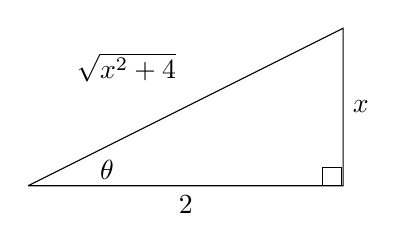
\begin{tikzpicture}
        \draw (0,0) node[above,right=1cm,above=-0.05cm] {$\theta$} -- node[below] {2} (4,0) node[draw,left=4pt,above=-0.25pt]{} -- node[right] {$x$} (4,2) -- node [above=0.5cm,left=0cm] {$\sqrt{x^2+4}$} (0,0);
      \end{tikzpicture}
    \end{center}
    We want $\sin\theta$; from the triangle, that equals $\displaystyle\frac{x}{\sqrt{x^2+4}}$.
  \end{solution}
  \newpage
  \question
  Evaluate $\displaystyle\frac{d}{dx}\sin^{-1}(x^3)$.
  \begin{enumerate}[label=\alph*)]
    \item
    $\displaystyle\sin^{-1}(3x^2)+\frac{1}{\sqrt{1-x^2}}(x^3)$
    \item
    $\displaystyle\frac{3x^2}{\sqrt{1-x^6}}$    
    \item
    $-3x^2\csc(x^3)\cot(x^3)$
    \item
    I don't know
  \end{enumerate}
  \begin{solution}
    b) $\displaystyle\frac{3x^2}{\sqrt{1-x^6}}$
    
    We have $\displaystyle\frac{d}{dx}\sin^{-1}x=\frac{1}{\sqrt{1-x^2}}$. Thus, by the Chain Rule:
    $$\frac{d}{dx}\sin^{-1}(x^3)=\frac{1}{\sqrt{1-(x^3)^2}}\cdot 3x^2=\frac{3x^2}{\sqrt{1-x^6}}$$
  \end{solution}
  \newpage
  \question
  Evaluate $\displaystyle\int\frac{1}{\sqrt{-x^2-4x-21}}\,dx$.
  \begin{enumerate}[label=\alph*)]
    \item
    $\displaystyle\sin^{-1}\left(\frac{x-2}{\sqrt{17}}\right)+C$
    \item
    $\displaystyle\sin^{-1}\left(\frac{x+2}{\sqrt{17}}\right)+C$
    \item
    $\displaystyle\sin^{-1}\left(\frac{x+2}{5}\right)+C$
    \item
    I don't know
  \end{enumerate}
  \begin{solution}
    c) $\displaystyle\sin^{-1}\left(\frac{x+2}{5}\right)+C$
    
    Complete the square under the radical:
    $$-x^2-4x+21=-(x^2+4x)+21=-(x^2+4x+4)+21+4=-(x+2)^2+25$$
    Insert that into the original integral:
    $$\int\frac{1}{\sqrt{-x^2-4x-21}}\,dx=\int\frac{1}{\sqrt{25-(x+2)^2}}\,dx$$
    Do a $u$-substitution: $u=x+2$, $du=dx$.
    $$\int\frac{1}{\sqrt{25-(x+2)^2}}\,dx=\int\frac{1}{\sqrt{25-u^2}}\,du=\sin^{-1}\left(\frac{u}{5}\right)+C=\sin^{-1}\left(\frac{x+2}{5}\right)+C$$
  \end{solution}
  \newpage
  \question
  Evaluate $\displaystyle\int\frac{1}{2x^2-12x+26}\,dx$.
  \begin{enumerate}[label=\alph*)]
    \item
    $\displaystyle\frac{1}{2}\tan^{-1}\left(\frac{x-3}{2}\right)+C$    
    \item
    $\displaystyle\frac{1}{4}\tan^{-1}\left(\frac{x-3}{2}\right)+C$
    \item
    $\displaystyle\frac{1}{2\sqrt{22}}\tan^{-1}\left(\frac{x-3}{\sqrt{22}}\right)+C$
    \item
    I don't know
  \end{enumerate}
  \begin{solution}
    b) $\displaystyle\frac{1}{4}\tan^{-1}\left(\frac{x-3}{2}\right)+C$
    
    $$\int\frac{1}{2x^2-12x+26}\,dx=\frac{1}{2}\int\frac{1}{x^2-6x+13}$$    
    Complete the square in denominator:
    $$x^2-6x+13=(x^2-6x+9)+13-9=(x-3)^2+4$$
    Insert that into the previous integral:
    $$\frac{1}{2}\int\frac{1}{x^2-6x+13}\,dx=\frac{1}{2}\int\frac{1}{(x-3)^2+4}\,dx$$
    Do a $u$-substitution: $u=x-3$, $du=dx$.
    $$\frac{1}{2}\int\frac{1}{(x-3)^2+4}\,dx=\frac{1}{2}\int\frac{1}{u^2+4}\,du=\frac{1}{2}\cdot\frac{1}{2}\tan^{-1}\left(\frac{u}{2}\right)+C=\frac{1}{4}\tan^{-1}\left(\frac{x-3}{2}\right)+C$$
  \end{solution}
  \newpage
  \question
  Which of the following expressions is equal to $\sinh^2 x+\cosh^2 x$?
  \begin{enumerate}[label=\alph*)]
    \item
    $\sinh 2x$
    \item
    $\cosh 2x$
    \item
    1
    \item
    I don't know
  \end{enumerate}
  \begin{solution}
    b) $\cosh 2x$
    
    $$\sinh^2 x+\cosh^2 x=\left(\frac{e^x-e^{-x}}{2}\right)^2+\left(\frac{e^x+e^{-x}}{2}\right)^2$$
    $$=\frac{e^{2x}-2+e^{-2x}}{4}+\frac{e^{2x}+2+e^{-2x}}{4}=\frac{2e^{2x}+2e^{-2x}}{4}=\frac{e^{2x}+e^{-2x}}{2}=\cosh 2x$$
  \end{solution}
  \newpage
  \question
  Which of the following expressions is equal to $\displaystyle\frac{e^{5x}+e^{-5x}}{e^{5x}-e^{-5x}}$?
  \begin{enumerate}[label=\alph*)]
    \item
    $\coth 5x$
    \item
    $\tanh 5x$
    \item
    $\mathrm{csch} \, 5x$
    \item
    I don't know
  \end{enumerate}
  \begin{solution}
    a) $\coth 5x$
    
    $$\coth 5x=\frac{\cosh 5x}{\sinh 5x}=\frac{\frac{1}{2}(e^{5x}+e^{-5x})}{\frac{1}{2}(e^{5x}-e^{-5x})}=\frac{e^{5x}+e^{-5x}}{e^{5x}-e^{-5x}}$$
  \end{solution}
  \newpage
  \question
  Evaluate $\displaystyle\int e^{4x}\sinh 7x\,dx$.
  \begin{enumerate}[label=\alph*)]
    \item
    $\displaystyle\frac{1}{24}e^{12x}+\frac{1}{4}e^{-2x}+C$
    \item
    $\displaystyle\frac{1}{22}e^{11x}+\frac{1}{6}e^{-3x}+C$
    \item
    $\displaystyle\frac{1}{56}e^{28x}+\frac{1}{56}e^{-28x}+C$
    \item
    I don't know
  \end{enumerate}
  \begin{solution}
    b) $\displaystyle\frac{1}{22}e^{11x}+\frac{1}{6}e^{-3x}+C$
    
    $$\int e^{4x}\sinh 7x\,dx=\int e^{4x}\left(\frac{e^{7x}-e^{-7x}}{2}\right)\,dx=\frac{1}{2}\int(e^{11x}-e^{-3x})\,dx$$
    $$=\frac{1}{2}\left(\frac{1}{11}e^{11x}+\frac{1}{3}e^{-3x}\right)+C=\frac{1}{22}e^{11x}+\frac{1}{6}e^{-3x}+C$$
  \end{solution}
  \newpage
\uplevel{Techniques of Integration}
  \question
  Evaluate $\displaystyle\int x^2 e^{3x}\,dx$.
  \begin{enumerate}[label=\alph*)]
    \item
    $\displaystyle x^2 e^{3x}-2x e^{3x}+2e^{3x}+C$
    \item
    $\displaystyle 3x^2 e^{3x}-18x e^{3x}+54e^{3x}+C$
    \item
    $\displaystyle\frac{1}{3}x^2 e^{3x}-\frac{2}{9}x e^{3x}+\frac{2}{27}e^{3x}+C$
    \item
    I don't know
  \end{enumerate}
  \begin{solution}
    c) $\displaystyle\frac{1}{3}x^2 e^{3x}-\frac{2}{9}x e^{3x}+\frac{2}{27}e^{3x}+C$
    
    You can integrate by parts twice, or you can save yourself some writing and use the tic-tac-toe method.
    \begin{center}
    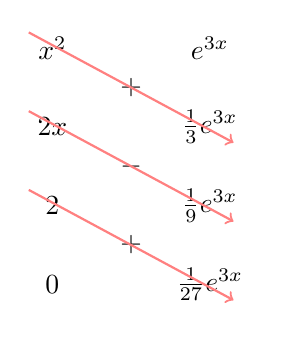
\begin{tikzpicture}
    \node at (0,0) {$x^2$};
    \node at (0,-1) {$2x$};
    \node at (0,-2) {2};
    \node at (0,-3) {0};
      
    \node at (2,0) {$e^{3x}$};
    \node at (2,-1) {$\frac{1}{3}e^{3x}$};
    \node at (2,-2) {$\frac{1}{9}e^{3x}$};
    \node at (2,-3) {$\frac{1}{27}e^{3x}$};
    
    \node at (1,-0.5) {$+$};
    \node at (1,-1.5) {$-$};
    \node at (1,-2.5) {$+$};
    
    \draw[->,red!50,thick] (-0.3,0.2) -- (2.3,-1.2);
    \draw[->,red!50,thick] (-0.3,-0.8) -- (2.3,-2.2);
    \draw[->,red!50,thick] (-0.3,-1.8) -- (2.3,-3.2);
    \end{tikzpicture}
    \end{center}
    $$\int x^2 e^{3x}\,dx=\frac{1}{3}x^2 e^{3x}-\frac{2}{9}x e^{3x}+\frac{2}{27}e^{3x}+C$$
  \end{solution}
  \newpage
  \question
  Evaluate $\displaystyle\int x^3\ln x\,dx$.
  \begin{enumerate}[label=\alph*)]
    \item
    $\displaystyle-\frac{1}{2}x^2+C$
    \item
    $\displaystyle\frac{1}{4}x^4\ln x-\frac{1}{16}x^4+C$    
    \item
    $\displaystyle\left(\frac{1}{4}x^4\right)\left(\frac{1}{x}\right)+C$
    \item
    I don't know
  \end{enumerate}
  \begin{solution}
    b) $\displaystyle\frac{1}{4}x^4\ln x-\frac{1}{16}x^4+C$
    
    Integrate by parts.
    $$u=\ln x; dv=x^3\,dx; du=\frac{1}{x}\,dx; v=\frac{1}{4}x^4$$
    $$\int x^3\ln x\,dx=\frac{1}{4}x^4\ln x-\int\left(\frac{1}{4}x^4\right)\left(\frac{1}{x}\,dx\right)=\frac{1}{4}x^4\ln x-\int\frac{1}{4}x^3\,dx$$
    $$=\frac{1}{4}x^4\ln x-\frac{1}{16}x^4+C$$
  \end{solution}
  \newpage
  \question
  Evaluate $\displaystyle\int x^3\cos(x^2)\,dx$.
  \begin{enumerate}[label=\alph*)]
    \item
    $\displaystyle\frac{1}{3}\sin(x^3)+C$
    \item
    $\displaystyle\frac{1}{2}x^2\cos(x^2)-\frac{1}{2}\sin(x^2)+C$
    \item
    $\displaystyle\frac{1}{2}x^2\sin(x^2)+\frac{1}{2}\cos(x^2)+C$
    \item
    I don't know
  \end{enumerate}
  \begin{solution}
    c) $\displaystyle\frac{1}{2}x^2\sin(x^2)+\frac{1}{2}\cos(x^2)+C$
    
    Start with a substitution:    
    $$z=x^2; dz=2x\,dx$$
    $$\int x^3\cos(x^2)\,dx=\int x^2(\cos (x^2))(x\,dx)=\frac{1}{2}\int z\cos z\,dz$$
    Now, integrate by parts:
    $$u=z; dv=\cos z\,dz; du=dz; v=\sin z$$
    $$\frac{1}{2}\int z\cos z\,dz=\frac{1}{2}\left(z\sin z-\int\sin z\,dz\right)=\frac{1}{2}(z\sin z+\cos z)+C$$
    $$=\frac{1}{2}\left(x^2\sin(x^2)+\cos(x^2)\right)+C$$
  \end{solution}
  \newpage
  \question
  Evaluate $\displaystyle\int(\sin^4 x)(\cos^5 x)\,dx$.
  \begin{enumerate}[label=\alph*)]
    \item
    $\displaystyle\frac{1}{9}\sin^9 x-\frac{2}{7}\sin^7 x+\frac{1}{5}\sin^5 x+C$
    \item
    $\displaystyle\frac{1}{5}\sin^5 x-\frac{1}{9}\sin^9 x+C$
    \item
    $\displaystyle\frac{1}{9}\cos^9 x-\frac{1}{6}\cos^6 x+C$
    \item
    I don't know
  \end{enumerate}
  \begin{solution}
    a) $\displaystyle\frac{1}{9}\sin^9 x-\frac{2}{7}\sin^7 x+\frac{1}{5}\sin^5 x+C$
    
    $$u=\sin x; du=\cos x\,dx$$
    $$\int(\sin^4 x)(\cos^5 x)\,dx=\int(\sin^4 x)(\cos^4 x)(\cos x)\,dx$$
    $$=\int(\sin^4 x)(1-\sin^2 x)^2(\cos x)\,dx=\int u^4(1-u^2)^2\,du=\int u^4(u^4-2u^2+1)\,du$$
    $$=\int(u^8-2u^6+u^4)\,du=\frac{1}{9}u^9-\frac{2}{7}u^7+\frac{1}{5}u^5+C=\frac{1}{9}\sin^9 x-\frac{2}{7}\sin^7 x+\frac{1}{5}\sin^5 x+C$$
  \end{solution}
  \newpage
  \question
  Evaluate $\displaystyle\int(\sin^3 x)(\cos^6 x)\,dx$.
  \begin{enumerate}[label=\alph*)]
    \item
    $\displaystyle\frac{1}{7}\cos^7 x-\frac{1}{10}\cos^{10}x+C$
    \item
    $\displaystyle\frac{1}{7}\cos^7 x-\frac{1}{9}\cos^9 x+C$
    \item
    $\displaystyle\frac{1}{9}\cos^9 x-\frac{1}{7}\cos^7 x+C$
    \item
    I don't know
  \end{enumerate}
  \begin{solution}
    c) $\displaystyle\frac{1}{9}\cos^9 x-\frac{1}{7}\cos^7 x+C$
    
    $$u=\cos x; du=-\sin x\,dx$$
    $$\int(\sin^3 x)(\cos^6 x)\,dx=\int(\sin^2 x)(\cos^6 x)(\sin x)\,dx$$
    $$=\int(1-\cos^2 x)(\cos^6 x)(\sin x)\,dx=\int(1-u^2)(u^6)(-du)=\int(u^8-u^6)\,du$$
    $$=\frac{1}{9}u^9-\frac{1}{7}u^7+C=\frac{1}{9}\cos^9 x-\frac{1}{7}\cos^7 x+C$$
  \end{solution}
  \newpage
  \question
  Evaluate $\displaystyle\int(\tan^4 x)(\sec^6 x)\,dx$.
  \begin{enumerate}[label=\alph*)]
    \item
    $\displaystyle\frac{1}{9}\tan^9 x+\frac{2}{7}\tan^7 x+\frac{1}{5}\tan^5 x+C$
    \item
    $\displaystyle\frac{1}{11}\tan^{11}x+\frac{1}{5}\tan^5 x+C$
    \item
    $\displaystyle\frac{1}{9}\tan^9 x+\frac{1}{5}\tan^5 x+C$
    \item
    I don't know
  \end{enumerate}
  \begin{solution}
    a) $\displaystyle\frac{1}{9}\tan^9 x+\frac{2}{7}\tan^7 x+\frac{1}{5}\tan^5 x+C$
    
    $$u=\tan x; du=\sec^2 x\,dx$$
    $$\int(\tan^4 x)(\sec^6 x)\,dx=\int(\tan^4 x)(\sec^4 x)(\sec^2 x)\,dx$$
    $$=\int(\tan^4 x)(\tan^2 x+1)^2(\sec^2 x)\,dx=\int u^4(u^2+1)^2\,du=\int u^4(u^4+2u^2+1)\,dx$$
    $$=\int(u^8+2u^6+u^4)\,du=\frac{1}{9}u^9+\frac{2}{7}u^7+\frac{1}{5}u^5+C=\frac{1}{9}\tan^9 x+\frac{2}{7}\tan^7 x+\frac{1}{5}\tan^5 x+C$$
  \end{solution}
  \newpage
  \question
  Evaluate $\displaystyle\int(\tan^3 x)(\sec^5 x)\,dx$.
  \begin{enumerate}[label=\alph*)]
    \item
    $\displaystyle\frac{1}{7}\sec^7 x-\frac{1}{5}\sec^5 x+C$
    \item
    $\displaystyle\frac{1}{5}\sec^5 x-\frac{1}{7}\sec^7 x+C$
    \item
    $\displaystyle\frac{1}{9}\sec^9 x-\frac{1}{4}\sec^4 x+C$
    \item
    I don't know
  \end{enumerate}
  \begin{solution}
    a) $\displaystyle\frac{1}{7}\sec^7 x-\frac{1}{5}\sec^5 x+C$
    
    $$u=\sec x; du=\sec x\tan x\,dx$$
    $$\int(\tan^3 x)(\sec^5 x)\,dx=\int(\tan^2 x)(\sec^4 x)(\sec x\tan x)\,dx$$
    $$=\int(\sec^2 x-1)(\sec^4 x)(\sec x\tan x)\,dx=\int(u^2-1)(u^4)\,du=\int(u^6-u^4)\,du$$
    $$=\frac{1}{7}u^7-\frac{1}{5}u^5+C=\frac{1}{7}\sec^7 x-\frac{1}{5}\sec^5 x+C$$
  \end{solution}
  \newpage
  \question
  Evaluate $\displaystyle\int_{\pi/3}^{2\pi/3}\sqrt{1-\cos 6x}\,dx$.
  \begin{enumerate}[label=\alph*)]
    \item
    $\displaystyle -\frac{2\sqrt{2}}{3}$
    \item
    $\displaystyle\frac{\sqrt{2}}{3}$
    \item
    $\displaystyle\frac{2\sqrt{2}}{3}$
    \item
    I don't know
  \end{enumerate}
  \begin{solution}
    c) $\displaystyle\frac{2\sqrt{2}}{3}$
    
    $$u=3x; du=3\,dx; \frac{1}{3}\,du=dx$$
    $$x=\pi/3\rightarrow u=\pi; x=2\pi/3\rightarrow u=2\pi$$
    $$\displaystyle\int_{\pi/3}^{2\pi/3}\sqrt{1-\cos 6x}\,dx=\int_\pi^{2\pi}\frac{1}{3}\sqrt{1-\cos 2u}\,du=\int_\pi^{2\pi}\frac{1}{3}\sqrt{1-(1-2\sin^2 u)}\,du$$
    $$=\int_\pi^{2\pi}\frac{1}{3}\sqrt{2\sin^2 u}\,du=\int_\pi^{2\pi}\frac{\sqrt{2}}{3}\cdot|\sin u|\,du=\int_\pi^{2\pi}\frac{-\sqrt{2}}{3}\sin u\,du$$
    $$=\left[\frac{\sqrt{2}}{3}\cos u\right]_\pi^{2\pi}=\left(\frac{\sqrt{2}}{3}\cos 2\pi\right)-\left(\frac{\sqrt{2}}{3}\cos\pi\right)=\frac{\sqrt{2}}{3}-\left(-\frac{\sqrt{2}}{3}\right)=\frac{2\sqrt{2}}{3}$$
    Note: we include a negative sign when we remove the absolute value bars. That is necessary because, when $\pi<u<2\pi$, $\sin u$ is negative.
  \end{solution}
  \newpage
  \question
  Evaluate $\displaystyle\int_{3\pi/4}^{\pi}\sqrt{1+\cos 4x}\,dx$.
  \begin{enumerate}[label=\alph*)]
    \item
    $-\sqrt{2}$
    \item
    $\displaystyle\frac{\sqrt{2}}{2}$
    \item
    $\sqrt{2}$
    \item
    I don't know
  \end{enumerate}
  \begin{solution}
    b) $\displaystyle\frac{\sqrt{2}}{2}$
    
    $$u=2x; du=2\,dx; \frac{1}{2}\,du=dx$$
    $$x=3\pi/4\rightarrow u=3\pi/2; x=\pi\rightarrow u=2\pi$$
    $$\displaystyle\int_{3\pi/4}^{\pi}\sqrt{1+\cos 4x}\,dx=\int_{3\pi/2}^{2\pi}\frac{1}{2}\sqrt{1+\cos 2u}\,du=\int_{3\pi/2}^{2\pi}\frac{1}{2}\sqrt{1+2\cos^2 u-1}\,du$$
    $$=\int_{3\pi/2}^{2\pi}\frac{1}{2}\sqrt{2\cos^2 u}\,du=\int_{3\pi/2}^{2\pi}\frac{\sqrt{2}}{2}\cdot|\cos u|\,du=\int_{3\pi/2}^{2\pi}\frac{\sqrt{2}}{2}\cos u\,du$$
    $$=\left[\frac{\sqrt{2}}{2}\sin u\right]_{3\pi/2}^{2\pi}=\left(\frac{\sqrt{2}}{2}\sin 2\pi\right)-\left(\frac{\sqrt{2}}{2}\sin\frac{3\pi}{2}\right)=0-\left(-\frac{\sqrt{2}}{2}\right)=\frac{\sqrt{2}}{2}$$
    Note: we can freely remove the absolute value bars here because, when $3\pi/2<u<2\pi$, $\cos u$ is positive.
  \end{solution}
  \newpage
  \question
  Evaluate $\displaystyle\int\frac{x^2}{(4-x^2)^{3/2}}\,dx$.
  \begin{enumerate}[label=\alph*)]
    \item
    $\displaystyle\frac{2x}{\sqrt{4-x^2}}-\left(2\sin^{-1}\frac{x}{2}\right)+C$
    \item
    $\displaystyle\frac{x}{\sqrt{4-x^2}}-\left(\sin^{-1}\frac{x}{2}\right)+C$
    \item
    $\displaystyle\frac{4}{\sqrt{4-x^2}}-\left(2\sin^{-1}\frac{x}{2}\right)+C$
    \item
    I don't know
  \end{enumerate}
  \begin{solution}
    b) $\displaystyle\frac{x}{\sqrt{4-x^2}}-\left(\sin^{-1}\frac{x}{2}\right)+C$
    
    Use a trig substitution:    
    $$x=2\sin\theta; dx=2\cos\theta\,d\theta$$
    $$\int\frac{x^2}{(4-x^2)^{3/2}}\,dx=\int\frac{4\sin^2\theta}{(4-4\sin^2\theta)^{3/2}}\cdot 2\cos\theta\,d\theta=\int\frac{4\sin^2\theta}{(4\cos^2\theta)^{3/2}}\cdot 2\cos\theta\,d\theta$$
    $$=\int\frac{4\sin^2\theta}{8\cos^3\theta}\cdot 2\cos\theta\,d\theta=\int\frac{\sin^2\theta}{\cos^2\theta}\,d\theta=\int\tan^2\theta\,d\theta$$
    $$=\int(\sec^2\theta-1)\,d\theta=\tan\theta-\theta+C=\frac{x}{\sqrt{4-x^2}}-\left(\sin^{-1}\frac{x}{2}\right)+C$$
    The last equality comes from a reference triangle. Since we have $\displaystyle\sin\theta=\frac{x}{2}$, we can set up a right triangle where one angle is $\theta$, the side opposite is $x$, and the hypotenuse is 2. The adjacent side is then $\sqrt{4-x^2}$ (by the Pythagorean Theorem), which gives us $\displaystyle\tan\theta=\frac{x}{\sqrt{4-x^2}}$.
    \begin{center}
      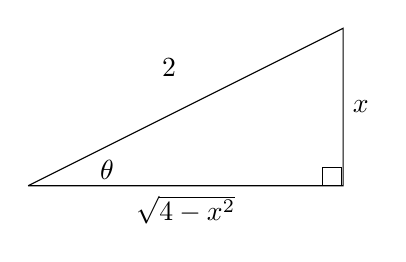
\begin{tikzpicture}
        \draw (0,0) node[above,right=1cm,above=-0.05cm] {$\theta$} -- node[below] {$\sqrt{4-x^2}$} (4,0) node[draw,left=4pt,above=-0.25pt]{} -- node[right] {$x$} (4,2) -- node [above=0.5cm,left=0cm] {2} (0,0);
      \end{tikzpicture}
    \end{center}
  \end{solution}
  \newpage
  \question
  Evaluate $\displaystyle\int\frac{1}{(x^2+9)^{3/2}}\,dx$.
  \begin{enumerate}[label=\alph*)]
    \item
    $\displaystyle\frac{x}{9\sqrt{x^2+9}}+C$
    \item
    $\displaystyle\frac{1}{3\sqrt{x^2+9}}+C$
    \item
    $\displaystyle\ln|(x^2+9)^{3/2}|+C$
    \item
    I don't know
  \end{enumerate}
  \begin{solution}
    a) $\displaystyle\frac{x}{9\sqrt{x^2+9}}+C$
    
    Use a trig substitution:    
    $$x=3\tan\theta; dx=3\sec^2\theta\,d\theta$$
    $$\int\frac{1}{(x^2+9)^{3/2}}\,dx=\int\frac{1}{(9\tan^2\theta+9)^{3/2}}\cdot 3\sec^2\theta\,d\theta=\int\frac{1}{(9\sec^2\theta)^{3/2}}\cdot 3\sec^2\theta\,d\theta$$
    $$=\int\frac{1}{27\sec^3\theta}\cdot 3\sec^2\theta\,d\theta=\frac{1}{9}\int\frac{1}{\sec\theta}\,d\theta=\frac{1}{9}\int\cos\theta\,d\theta$$
    $$=\frac{1}{9}\sin\theta+C=\frac{1}{9}\left(\frac{x}{\sqrt{x^2+9}}\right)+C$$
    The last equality comes from a reference triangle. Since we have $\displaystyle\tan\theta=\frac{x}{3}$, we can set up a right triangle where one angle is $\theta$, the side opposite is $x$, and the side adjacent is 3. The hypotenuse is then $\sqrt{x^2+9}$ (by the Pythagorean Theorem), which gives us $\displaystyle\sin\theta=\frac{x}{\sqrt{x^2+9}}$.
    \begin{center}
      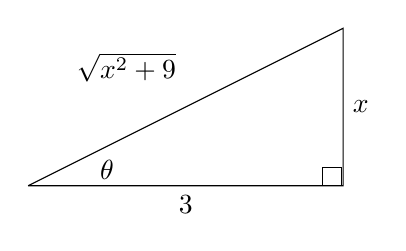
\begin{tikzpicture}
        \draw (0,0) node[above,right=1cm,above=-0.05cm] {$\theta$} -- node[below] {3} (4,0) node[draw,left=4pt,above=-0.25pt]{} -- node[right] {$x$} (4,2) -- node [above=0.5cm,left=0cm] {$\sqrt{x^2+9}$} (0,0);
      \end{tikzpicture}
    \end{center}
  \end{solution}
  \newpage
  \question
  Evaluate $\displaystyle\int\frac{\sqrt{x^2-16}}{x}\,dx$, assuming that $x>4$.
  \begin{enumerate}[label=\alph*)]
    \item
    $\displaystyle\sqrt{x^2-16}-4x+C$
    \item
    $\displaystyle\sqrt{x^2-16}-\left(4\sec^{-1}\frac{x}{4}\right)+C$
    \item
    $\displaystyle x-4\ln|x|+C$
    \item
    I don't know
  \end{enumerate}
  \begin{solution}
    b) $\displaystyle\sqrt{x^2-16}-\left(4\sec^{-1}\frac{x}{4}\right)+C$
    
    Use a trig substitution:    
    $$x=4\sec\theta; dx=4\sec\theta\tan\theta\,d\theta$$
    $$\int\frac{\sqrt{x^2-16}}{x}\,dx=\int\frac{\sqrt{16\sec^2\theta-16}}{4\sec\theta}(4\sec\theta\tan\theta)\,d\theta$$
    $$=\int\left(\sqrt{16\sec^2\theta-16}\right)(\tan\theta)\,d\theta=\int\left(\sqrt{16\tan^2\theta}\right)(\tan\theta)\,d\theta=\int(4\tan\theta)(\tan\theta)\,d\theta$$
    Note: in order to replace $\sqrt{16\tan^2\theta}$ with $4\tan\theta$ instead of $4|\tan\theta|$, we had to know that $x>4$.
    $$=4\int(\tan^2\theta)\,d\theta=4\int(\sec^2\theta-1)\,d\theta=4(\tan\theta-\theta)+C=4\left(\frac{\sqrt{x^2-16}}{4}-\sec^{-1}\frac{x}{4}\right)+C$$
    The last equality comes from a reference triangle. Since we have $\displaystyle\sec\theta=\frac{x}{4}$, we can set up a right triangle where one angle is $\theta$, the hypotenuse is $x$, and the side adjacent is 4. The opposite side is then $\sqrt{x^2-16}$ (by the Pythagorean Theorem), which gives us $\displaystyle\tan\theta=\frac{\sqrt{x^2-16}}{4}$.
    \begin{center}
      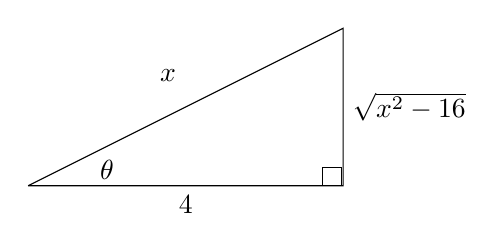
\begin{tikzpicture}
        \draw (0,0) node[above,right=1cm,above=-0.05cm] {$\theta$} -- node[below] {4} (4,0) node[draw,left=4pt,above=-0.25pt]{} -- node[right] {$\sqrt{x^2-16}$} (4,2) -- node [above=0.4cm,left=0cm] {$x$} (0,0);
      \end{tikzpicture}
    \end{center}
  \end{solution}
  \newpage
  \question
  Evaluate $\displaystyle\int\frac{3x+17}{x^2-5x-6}\,dx$.
  \begin{enumerate}[label=\alph*)]
    \item
    $-23\ln|x-2|+26\ln|x-3|+C$
    \item
    $-2\ln|x+1|+5\ln|x-6|+C$
    \item
    $5\ln|x+1|-2\ln|x-6|+C$
    \item
    I don't know
  \end{enumerate}
  \begin{solution}
    b) $-2\ln|x+1|+5\ln|x-6|+C$
    
    Use partial fractions:
    $$\int\frac{3x+17}{x^2-5x-6}\,dx=\int\frac{3x+17}{(x+1)(x-6)}\,dx=\int\left(\frac{A}{x+1}+\frac{B}{x-6}\right)\,dx$$
    $$3x+17=A(x-6)+B(x+1)$$
    Plug in $x=-1$:
    $$14=A(-7)$$
    $$A=-2$$    
    Plug in $x=6$:
    $$35=B(7)$$
    $$B=5$$
    Back to the original integral:
    $$\int\left(\frac{-2}{x+1}+\frac{5}{x-6}\right)\,dx=-2\ln|x+1|+5\ln|x-6|+C$$
  \end{solution}
  \newpage
  \question
  Evaluate $\displaystyle\int\frac{1}{x^3+x^2}\,dx$.
  \begin{enumerate}[label=\alph*)]
    \item
    $-\ln|x|+\ln|x^2|+\ln|x+1|+C$
    \item
    $\displaystyle -\ln|x|-\frac{1}{x}+\ln|x+1|+C$
    \item
    $\ln|x^2|+\ln|x+1|+C$
    \item
    I don't know
  \end{enumerate}
  \begin{solution}
    b) $\displaystyle -\ln|x|-\frac{1}{x}+\ln|x+1|+C$
    
    Use partial fractions:
    $$\int\frac{1}{x^3+x^2}\,dx=\int\frac{1}{x^2(x+1)}\,dx=\int\left(\frac{A}{x}+\frac{B}{x^2}+\frac{C}{x+1}\right)\,dx$$
    $$1=Ax(x+1)+B(x+1)+Cx^2$$
    Plug in $x=0$: $1=B$
    
    Plug in $x=-1$: $1=C$
    
    Plug those values for $B$ and $C$ into our equation:
    $$1=Ax(x+1)+x+1+x^2$$
    Plug in $x=1$:
    $$1=2A+1+1+1$$
    $$A=-1$$
    Back to the original integral:
    $$\int\left(\frac{-1}{x}+\frac{1}{x^2}+\frac{1}{x+1}\right)\,dx=-\ln|x|-\frac{1}{x}+\ln|x+1|+C$$
  \end{solution}
  \newpage
  \question
  Evaluate $\displaystyle\int\frac{\sqrt{x}}{x+16}\,dx$.
  \begin{enumerate}[label=\alph*)]
    \item
    $\displaystyle 2\sqrt{x}+\frac{1}{24}x\sqrt{x}+C$
    \item
    $\displaystyle 2\sqrt{x}-32\ln|x+16|+C$
    \item
    $\displaystyle 2\sqrt{x}-8\tan^{-1}\left(\frac{\sqrt{x}}{4}\right)+C$
    \item
    I don't know
  \end{enumerate}
  \begin{solution}
    c) $\displaystyle 2\sqrt{x}-8\tan^{-1}\left(\frac{\sqrt{x}}{4}\right)+C$
    
    Use a rationalizing substitution:
    $$u=\sqrt{x}; x=u^2; dx=2u\,du$$
    $$\int\frac{\sqrt{x}}{x+16}\,dx=\int\frac{u}{u^2+16}\cdot 2u\,du=\int\frac{2u^2}{u^2+16}\,du$$
    $$=\int\frac{2u^2+32-32}{u^2+16}\,du=\int\left(2-\frac{32}{u^2+16}\right)\,du$$
    $$=2u-32\cdot\frac{1}{4}\tan^{-1}\left(\frac{u}{4}\right)+C=2\sqrt{x}-8\tan^{-1}\left(\frac{\sqrt{x}}{4}\right)+C$$
  \end{solution}
  \newpage
  \question
  Evaluate $\displaystyle\int\frac{3x^2+10}{x-2}\,dx$.
  \begin{enumerate}[label=\alph*)]
    \item
    $\displaystyle\frac{3}{2}x^2-5x+C$
    \item
    $\displaystyle\frac{3}{2}x^2-6x-2\ln|x-2|+C$
    \item
    $\displaystyle\frac{3}{2}x^2+6x+22\ln|x-2|+C$
    \item
    I don't know
  \end{enumerate}
  \begin{solution}
    c) $\displaystyle\frac{3}{2}x^2+6x+22\ln|x-2|+C$
    
    Use long division:
    $$\polylongdiv{3x^2+10}{x-2}$$
    $$\int\frac{3x^2+10}{x-2}\,dx=\int\left(3x+6+\frac{22}{x-2}\right)\,dx=\frac{3}{2}x^2+6x+22\ln|x-2|+C$$
  \end{solution}
  \newpage
  \question
  Use the Trapezoidal Method with $n=6$ subintervals to approximate $\displaystyle\int_3^{15}\ln x\,dx$. Round off your answer to two places after the decimal point.
  \begin{enumerate}[label=\alph*)]
    \item
    25.24
    \item
    25.28
    \item
    25.32
    \item
    I don't know
  \end{enumerate}
  \begin{solution}
    a) 25.24
    
    Let $f(x)=\ln x$, the function being integrated.
    
    Find the width of each subinterval. If the endpoints are $a$ and $b$ and the number of subintervals is $n$, then the width is:
    $$\frac{b-a}{n}=\frac{15-3}{6}=2$$
    Find the endpoints of the subintervals, starting from $a=3$ and moving forward by one width (2 units) at each step: 
    $$x_0=3, x_1=5, x_2=7, x_3=9, x_4=11, x_5=13, x_6=15$$
    Here's the approximation:
    $$\int_3^{15}\ln x\,dx\approx\frac{b-a}{2n}(f(3)+2f(5)+2f(7)+2f(9)+2f(11)+2f(13)+f(15))$$
    $$=1\cdot(\ln 3+2\ln 5+2\ln 7+2\ln 9+2\ln 11+2\ln 13+\ln 15)\approx 25.24$$
  \end{solution}
  \newpage
  \question
  Use Simpson's Method with $n=4$ subintervals to approximate $\displaystyle\int_{-1}^5 xe^x\,dx$. Round off your answer to two places after the decimal point.
  \begin{enumerate}[label=\alph*)]
    \item
    594.39    
    \item
    619.08
    \item
    753.53
    \item
    I don't know
  \end{enumerate}
  \begin{solution}
    b) 619.08
    
    Let $f(x)=xe^x$, the function being integrated.
    
    Find the width of each subinterval. If the endpoints are $a$ and $b$ and the number of subintervals is $n$, then the width is:
    $$\frac{b-a}{n}=\frac{5-(-1)}{4}=1.5$$
    Find the endpoints of the subintervals, starting from $a=-1$ and moving forward by one width (1.5 units) at each step: 
    $$x_0=-1, x_1=0.5, x_2=2, x_3=3.5, x_4=5$$
    Here's the approximation:
    $$\int_{-1}^5 xe^x\,dx\approx\frac{b-a}{3n}(f(-1)+4f(0.5)+2f(2)+4f(3.5)+f(5))$$
    $$=0.5\cdot\left(-e^{-1}+4\cdot 0.5e^{0.5}+2\cdot 2e^2+4\cdot 3.5e^{3.5}+5e^5\right)\approx 619.08$$
  \end{solution}
  \newpage
  \question
  Determine whether the integral $\displaystyle\int_5^\infty\frac{1}{x(\ln x)^3}\,dx$ converges or diverges. If it converges, find what it converges to.
  \begin{enumerate}[label=\alph*)]
    \item
    converges to $\displaystyle\frac{1}{4(\ln 5)^4}$
    \item
    converges to $\displaystyle\frac{1}{2(\ln 5)^2}$
    \item
    diverges
    \item
    I don't know
  \end{enumerate}
  \begin{solution}
    b) converges to $\displaystyle\frac{1}{2(\ln 5)^2}$
    
    $$\int_5^\infty\frac{1}{x(\ln x)^3}\,dx=\lim_{b\to\infty}\int_5^b\frac{1}{x(\ln x)^3}\,dx$$
    $$u=\ln x; du=\frac{1}{x}\,dx$$
    $$x=5\rightarrow u=\ln 5$$
    $$x=b\rightarrow u=\ln b$$
    $$\lim_{b\to\infty}\int_{\ln 5}^{\ln b}\frac{1}{u^3}\,du=\lim_{b\to\infty}\int_{\ln 5}^{\ln b}u^{-3}\,du=\lim_{b\to\infty}\left[-\frac{1}{2}u^{-2}\right]_{\ln 5}^{\ln b}$$
    $$=\lim_{b\to\infty}\left[\frac{-1}{2(\ln b)^2}-\frac{-1}{2(\ln 5)^2}\right]=0-\frac{-1}{2(\ln 5)^2}=\frac{1}{2(\ln 5)^2}$$
  \end{solution}
  \newpage
  \question
  Determine whether the integral $\displaystyle\int_{-\infty}^1\frac{1}{1+x^2}\,dx$ converges or diverges. If it converges, find what it converges to.
  \begin{enumerate}[label=\alph*)]
    \item
    converges to $\displaystyle\frac{\pi}{4}$
    \item
    converges to $\displaystyle\frac{3\pi}{4}$
    \item
    diverges
    \item
    I don't know
  \end{enumerate}
  \begin{solution}
    b) converges to $\displaystyle\frac{3\pi}{4}$
    
    $$\int_{-\infty}^1\frac{1}{1+x^2}\,dx=\lim_{a\to -\infty}\int_a^1\frac{1}{1+x^2}\,dx=\lim_{a\to -\infty}\left[\tan^{-1}x\right]_a^1$$
    $$=\lim_{a\to -\infty}(\tan^{-1}1-\tan^{-1}a)=\frac{\pi}{4}-\left(-\frac{\pi}{2}\right)=\frac{3\pi}{4}$$
  \end{solution}
  \newpage
  \question
  Determine whether the integral $\displaystyle\int_{-\infty}^\infty x^{1/3}\,dx$ converges or diverges. If it converges, find what it converges to.
  \begin{enumerate}[label=\alph*)]
    \item
    converges to 0
    \item
    converges to $\displaystyle\frac{3}{4}$
    \item
    diverges
    \item
    I don't know
  \end{enumerate}
  \begin{solution}
    c) diverges
    
    Split up the integral:
    $$\int_{-\infty}^\infty x^{1/3}\,dx=\int_{-\infty}^0 x^{1/3}\,dx+\int_0^\infty x^{1/3}\,dx$$
    Note that the breaking point does not need to be at $x=0$, but let's choose that point for simplicity.
    
    We can work with either piece first. Let's say we choose the second piece:
    $$\int_0^\infty x^{1/3}\,dx=\lim_{b\to\infty}\int_0^b x^{1/3}\,dx=\lim_{b\to\infty}\left[\frac{3}{4}x^{4/3}\right]_0^b$$
    $$=\lim_{b\to\infty}\left(\frac{3}{4}b^{4/3}-0\right)=\infty$$
    This piece diverges, so there is no need to check the other piece. We now know that $\displaystyle\int_{-\infty}^\infty x^{1/3}\,dx$ diverges.
  \end{solution}
  \newpage
  \question
  Determine whether the integral $\displaystyle\int_0^{16}\frac{3}{x^{1/4}}\,dx$ converges or diverges. If it converges, find what it converges to.
  \begin{enumerate}[label=\alph*)]
    \item
    converges to 18
    \item
    converges to 32
    \item
    diverges
    \item
    I don't know
  \end{enumerate}
  \begin{solution}
    b) converges to 32
    
    Note that this function has an infinite discontinuity at $x=0$, which is an endpoint of the interval. So we need a limit:
    $$\int_0^{16}\frac{3}{x^{1/4}}\,dx=\lim_{a\to 0^+}\int_a^{16} 3x^{-1/4}\,dx=\lim_{a\to 0^+}\left[3\cdot\frac{4}{3}x^{3/4}\right]_a^{16}$$
    $$=\lim_{a\to 0^+}4\left(16^{3/4}-a^{3/4}\right)=4(8-0)=32$$
  \end{solution}
  \newpage
  \question
  Determine whether the integral $\displaystyle\int_3^8\frac{1}{(x-5)^2}\,dx$ converges or diverges. If it converges, find what it converges to.
  \begin{enumerate}[label=\alph*)]
    \item
    converges to $\displaystyle -\frac{5}{6}$
    \item
    converges to $\displaystyle\frac{5}{36}$
    \item
    diverges
    \item
    I don't know
  \end{enumerate}
  \begin{solution}
    c) diverges
    
    Note that this function has an infinite discontinuity at $x=5$, which is inside the interval. So we need to split up the integral:
    $$\int_3^8\frac{1}{(x-5)^2}\,dx=\int_3^5\frac{1}{(x-5)^2}\,dx+\int_5^8\frac{1}{(x-5)^2}\,dx$$
    We can work with either piece first. Let's say we choose the first piece:
    $$\int_3^5\frac{1}{(x-5)^2}\,dx=\lim_{c\to 5^-}\int_3^c\frac{1}{(x-5)^2}\,dx=\lim_{c\to 5^-}\int_3^c (x-5)^{-2}\,dx$$
    $$=\lim_{c\to 5^-}\left[-(x-5)^{-1}\right]_3^c=\lim_{c\to 5^-}\left[\frac{-1}{c-5}-\frac{-1}{3-5}\right]=\infty-\frac{1}{2}=\infty$$
    This piece diverges, so there is no need to check the other piece. We now know that $\displaystyle\int_3^8\frac{1}{(x-5)^2}\,dx$ diverges.
  \end{solution}
  \newpage
  \question
  Let's say we want to determine whether the integral $\displaystyle\int_2^\infty\frac{4x^{1.5}+3}{x^3+5x}\,dx$ converges or diverges. We choose to compare that integral to the integral $\displaystyle\int_2^\infty\frac{1}{x^{1.5}}\,dx$, and we choose to use the Limit Comparison Test. What will be the result of that test?
  \begin{enumerate}[label=\alph*)]
    \item
    the test says that the original integral converges
    \item
    the test says that the original integral diverges
    \item
    the test is inconclusive
    \item
    I don't know
  \end{enumerate}
  \begin{solution}
    a) the test says that the original integral converges
    
    For any constants $a$ and $p$ (where $a>0$), the integral $\displaystyle\int_a^{\infty}\frac{1}{x^p}\,dx$ converges if and only if $p>1$. Thus, the integral $\displaystyle\int_2^\infty\frac{1}{x^{1.5}}\,dx$ converges; if the Limit Comparison Test is successful, the original integral will also converge.
    $$\lim_{x\to\infty}\frac{\left(\frac{4x^{1.5}+3}{x^3+5x}\right)}{\left(\frac{1}{x^{1.5}}\right)}=\lim_{x\to\infty}\left(\frac{4x^{1.5}+3}{x^3+5x}\right)\cdot x^{1.5}=\lim_{x\to\infty}\frac{4x^3+3x^{1.5}}{x^3+5x}=\frac{4}{1}=4$$
    We got a result greater than 0 and less than $\infty$, so the test was successful. Since $\displaystyle\int_2^\infty\frac{1}{x^{1.5}}\,dx$ converges, $\displaystyle\int_2^\infty\frac{4x^{1.5}+3}{x^3+5x}\,dx$ must also converge.
  \end{solution}
  \newpage
  \question
  Let's say we want to determine whether the integral $\displaystyle\int_1^\infty\frac{7x^2-4x}{x^{2.5}+9}\,dx$ converges or diverges. We choose to compare that integral to the integral $\displaystyle\int_1^\infty\frac{1}{x^{0.5}}\,dx$, and we choose to use the Limit Comparison Test. What will be the result of that test?
  \begin{enumerate}[label=\alph*)]
    \item
    the test says that the original integral converges
    \item
    the test says that the original integral diverges
    \item
    the test is inconclusive
    \item
    I don't know
  \end{enumerate}
  \begin{solution}
    b) the test says that the original integral diverges
    
    For any constants $a$ and $p$ (where $a>0$), the integral $\displaystyle\int_a^{\infty}\frac{1}{x^p}\,dx$ converges if and only if $p>1$. Thus, the integral $\displaystyle\int_1^\infty\frac{1}{x^{0.5}}\,dx$ diverges; if the Limit Comparison Test is successful, the original integral will also diverge.
    $$\lim_{x\to\infty}\frac{\left(\frac{7x^2-4x}{x^{2.5}+9}\right)}{\left(\frac{1}{x^{0.5}}\right)}=\lim_{x\to\infty}\left(\frac{7x^2-4x}{x^{2.5}+9}\right)\cdot x^{0.5}=\lim_{x\to\infty}\frac{7x^{2.5}-4x^{1.5}}{x^{2.5}+9}=\frac{7}{1}=7$$
    We got a result greater than 0 and less than $\infty$, so the test was successful. Since $\displaystyle\int_1^\infty\frac{1}{x^{0.5}}\,dx$ diverges, $\displaystyle\int_1^\infty\frac{7x^2-4x}{x^{2.5}+9}\,dx$ must also diverge.
  \end{solution}
  \newpage
  \question
  Let's say we want to determine whether the integral $\displaystyle\int_4^\infty\frac{2+\cos x}{x}\,dx$ converges or diverges. We choose to compare that integral to the integral $\displaystyle\int_4^\infty\frac{1}{x}\,dx$, and we choose to use the Limit Comparison Test. What will be the result of that test?
  \begin{enumerate}[label=\alph*)]
    \item
    the test says that the original integral converges
    \item
    the test says that the original integral diverges
    \item
    the test is inconclusive
    \item
    I don't know
  \end{enumerate}
  \begin{solution}
    c) the test is inconclusive
    
    For any constants $a$ and $p$ (where $a>0$), the integral $\displaystyle\int_a^{\infty}\frac{1}{x^p}\,dx$ converges if and only if $p>1$. Thus, the integral $\displaystyle\int_4^\infty\frac{1}{x}\,dx$ diverges; if the Limit Comparison Test is successful, the original integral will also diverge.
    $$\lim_{x\to\infty}\frac{\left(\frac{2+\cos x}{x}\right)}{\left(\frac{1}{x}\right)}=\lim_{x\to\infty}(2+\cos x)$$
    This limit doesn't exist, so the test is inconclusive.
  \end{solution}
  \newpage
  \question
  Let's say we want to determine whether the integral $\displaystyle\int_1^\infty\frac{3+\sin x}{x^2}\,dx$ converges or diverges. We choose to compare that integral to the integral $\displaystyle\int_1^\infty \frac{4}{x^2}\,dx$, and we choose to use the Direct Comparison Test. What will be the result of that test?
  \begin{enumerate}[label=\alph*)]
    \item
    the test says that the original integral converges
    \item
    the test says that the original integral diverges
    \item
    the test is inconclusive
    \item
    I don't know
  \end{enumerate}
  \begin{solution}
    a) the test says that the original integral converges
    
    For any constants $a$ and $p$ (where $a>0$), the integral $\displaystyle\int_a^{\infty}\frac{1}{x^p}\,dx$ converges if and only if $p>1$. Thus, the integral $\displaystyle\int_1^\infty\frac{1}{x^2}\,dx$ converges; so does $\displaystyle\int_1^\infty\frac{4}{x^2}\,dx$, which is four times as large.
    
    We have $\displaystyle 0<\frac{3+\sin x}{x^2}\le\frac{4}{x^2}$ for all $x\ge 1$. Since $\displaystyle\int_1^\infty\frac{4}{x^2}\,dx$ converges, and $\displaystyle\frac{3+\sin x}{x^2}$ is a lesser function, it must be that $\displaystyle\int_1^\infty\frac{3+\sin x}{x^2}\,dx$ also converges.
  \end{solution}
  \newpage
  \question
  Let's say we want to determine whether the integral $\displaystyle\int_5^\infty\frac{1}{x^{0.9}(\ln x)^7}\,dx$ converges or diverges. We choose to compare that integral to the integral $\displaystyle\int_5^\infty\frac{1}{x^{0.91}}\,dx$, and we choose to use the Direct Comparison Test. What will be the result of that test?
  \begin{enumerate}[label=\alph*)]
    \item
    the test says that the original integral converges
    \item
    the test says that the original integral diverges
    \item
    the test is inconclusive
    \item
    I don't know
  \end{enumerate}
  \begin{solution}
    b) the test says that the original integral diverges
    
    For any constants $a$ and $p$ (where $a>0$), the integral $\displaystyle\int_a^{\infty}\frac{1}{x^p}\,dx$ converges if and only if $p>1$. Thus, the integral $\displaystyle\int_5^\infty\frac{1}{x^{0.91}}\,dx$ diverges.
    
    Long-term, any positive power of the natural log function grows slower than any positive power of $x$. Thus, we have $(\ln x)^7<x^{0.01}$ for all sufficiently large $x$. And that means, for all sufficiently large $x$, we have:
    $$\frac{1}{x^{0.9}(\ln x)^7}>\frac{1}{x^{0.9}\cdot x^{0.01}}=\frac{1}{x^{0.91}}>0$$
    Since $\displaystyle\int_5^\infty\frac{1}{x^{0.91}}\,dx$ diverges, and $\displaystyle\frac{1}{x^{0.9}(\ln x)^7}$ is a greater function long-term, it must be that $\displaystyle\int_5^\infty\frac{1}{x^{0.9}(\ln x)^7}\,dx$ also diverges.
  \end{solution}
  \newpage
  \question
  Let's say we want to determine whether the integral $\displaystyle\int_3^\infty\frac{1}{x(\ln x)^2}\,dx$ converges or diverges. We choose to compare that integral to the integral $\displaystyle\int_3^\infty\frac{1}{x}\,dx$, and we choose to use the Direct Comparison Test. What will be the result of that test?
  \begin{enumerate}[label=\alph*)]
    \item
    the test says that the original integral converges
    \item
    the test says that the original integral diverges
    \item
    the test is inconclusive
    \item
    I don't know
  \end{enumerate}
  \begin{solution}
    c) the test is inconclusive
    
    For any constants $a$ and $p$ (where $a>0$), the integral $\displaystyle\int_a^{\infty}\frac{1}{x^p}\,dx$ converges if and only if $p>1$. Thus, the integral $\displaystyle\int_3^\infty\frac{1}{x}\,dx$ diverges.
    
    We have $\displaystyle 0<\frac{1}{x(\ln x)^2}<\frac{1}{x}$ for all $x\ge 3$. Unfortunately. having the greater integral diverge tells us nothing about the lesser integral. Thus, the test is inconclusive.
  \end{solution}
  \newpage
\uplevel{Separable Differential Equations}
  \question
  Find the function $y$ of $x$ satisfying the differential equation $\displaystyle\frac{dy}{dx}=e^{7x+4y}$ and the initial condition $y(0)=1$. Your answer does not need to be in the form $y=f(x)$; a general equation in $x$ and $y$ is okay.
  \begin{enumerate}[label=\alph*)]
    \item
    $\displaystyle \frac{1}{4}e^{4y}=-\frac{1}{7}e^{-7x}+\frac{1}{4}e^4+\frac{1}{7}$
    \item
    $\displaystyle \frac{1}{4}e^{4y}=\frac{1}{7}e^{7x}+\frac{1}{4}e^4-\frac{1}{7}$
    \item
    $\displaystyle -\frac{1}{4}e^{-4y}=\frac{1}{7}e^{7x}-\frac{1}{4}e^{-4}-\frac{1}{7}$
    \item
    I don't know
  \end{enumerate}
  \begin{solution}
    c) $\displaystyle -\frac{1}{4}e^{-4y}=\frac{1}{7}e^{7x}-\frac{1}{4}e^{-4}-\frac{1}{7}$
        
    $$\frac{dy}{dx}=e^{7x+4y}$$
    $$\frac{dy}{dx}=e^{7x}e^{4y}$$
    $$e^{-4y}\,dy=e^{7x}\,dx$$
    $$\int e^{-4y}\,dy=\int e^{7x}\,dx$$
    $$-\frac{1}{4}e^{-4y}=\frac{1}{7}e^{7x}+C$$
    Now, solve for the constant: 
    $$-\frac{1}{4}e^{-4}=\frac{1}{7}e^0+C$$
    $$-\frac{1}{4}e^{-4}=\frac{1}{7}+C$$
    $$-\frac{1}{4}e^{-4}-\frac{1}{7}=C$$
    We thus get our final solution:
    $$-\frac{1}{4}e^{-4y}=\frac{1}{7}e^{7x}-\frac{1}{4}e^{-4}-\frac{1}{7}$$
  \end{solution}
  \newpage
  \question
  Find the function $y$ of $x$ satisfying the differential equation $\displaystyle\frac{dy}{dx}=\frac{\tan y}{x}$ and the initial condition $\displaystyle y(-5)=\frac{\pi}{6}$. Your answer does not need to be in the form $y=f(x)$; a general equation in $x$ and $y$ is okay.
  \begin{enumerate}[label=\alph*)]
    \item
    $\displaystyle -\ln|\cos y|=\ln|x|-\ln\left(\frac{\sqrt{3}}{2}\right)-\ln 5$
    \item
    $\displaystyle\ln|\sin y|=\ln|x|+\ln\left(\frac{1}{2}\right)-\ln 5$
    \item
    $\displaystyle\frac{1}{2}x^2=-\ln|\cos y|+\frac{25}{2}+\ln\left(\frac{\sqrt{3}}{2}\right)$
    \item
    I don't know
  \end{enumerate}
  \begin{solution}
    b) $\displaystyle\ln|\sin y|=\ln|x|+\ln\left(\frac{1}{2}\right)-\ln 5$
    
    $$\frac{dy}{dx}=\frac{\tan y}{x}$$
    $$\cot y\,dy=\frac{1}{x}\,dx$$
    $$\int\cot y\,dy=\int\frac{1}{x}\,dx$$
    $$\ln|\sin y|=\ln|x|+C$$
    Now, solve for the constant: 
    $$\ln\left|\sin\frac{\pi}{6}\right|=\ln|-5|+C$$
    $$\ln\left(\frac{1}{2}\right)=\ln 5+C$$
    $$\ln\left(\frac{1}{2}\right)-\ln 5=C$$
    We thus get our final solution:
    $$\ln|\sin y|=\ln|x|+\ln\left(\frac{1}{2}\right)-\ln 5$$
  \end{solution}
  \newpage
  \question
  Let's say you open a savings account, with \$500 as your initial deposit. Assume that you don't make any deposits or withdrawals after that initial deposit. Also assume the interest is compounded continuously, and the interest rate never changes. If you have \$600 in the account 5 years after the initial deposit, then how much will you have 18 years after the initial deposit?
  \begin{enumerate}[label=\alph*)]
    \item
    \$860.00
    \item
    \$963.88
    \item
    \$1156.65
    \item
    I don't know
  \end{enumerate}
  \begin{solution}
    b) \$963.88
    
    The amount of money in the account follows the following formula:
    $$y=y_0e^{kt}$$
    Here, $t$ is the number of years elapsed, $y_0$ is the initial deposit, $y$ is the amount of money in the account at time $t$, and $k$ is the interest rate.
    
    In this case, we are given that $y_0=500$:
    $$y=500e^{kt}$$
    We have $y=600$ when $t=5$. Let's use that to solve for $k$:
    $$600=500e^{5k}$$
    $$1.2=e^{5k}$$
    $$5k=\ln 1.2$$
    $$k=\frac{1}{5}\ln 1.2$$
    Now we find the value of $y$ when $t=18$, and we're done:
    $$y=500e^{(1/5)(\ln 1.2)(18)}\approx 963.88$$
    You end up with \$963.88.
  \end{solution}
  \newpage
  \question
  Let's say we have a radioactive isotope which decays so quickly, that it only takes 9 days for 90\% of a sample to decay. What is the half-life (in days) of such an isotope? Round off your answer to two digits after the decimal point.
  \begin{enumerate}[label=\alph*)]
    \item
    0.26 days
    \item
    2.71 days
    \item
    59.21 days
    \item
    I don't know
  \end{enumerate}
  \begin{solution}
    b) 2.71 days
    
    Radioactive decay follows the following formula:
    $$y=y_0e^{kt}$$
    Here, $t$ is the time elapsed, $y_0$ is the initial mass of the sample, $y$ is the mass of the sample at time $t$, and $k$ is a constant depending on the half-life.
    
    When $t=9$, only 10\% of the sample is left, so $y=0.1y_0$. Let's use that to solve for $k$:
    $$0.1y_0=y_0e^{9k}$$
    $$0.1=e^{9k}$$
    $$9k=\ln 0.1$$
    $$k=\frac{1}{9}\ln 0.1$$
    Now, there is a formula connecting the value of $k$ to the half-life $h$: $\displaystyle k=\frac{\ln 0.5}{h}$. This can be rewritten as $\displaystyle h=\frac{\ln 0.5}{k}$. And with that, we can get the half-life:
    $$h=\frac{\ln 0.5}{\frac{1}{9}\ln 0.1}\approx 2.71\text{ days}$$
  \end{solution}
  \newpage
  \question
  I took a water bottle at a temperature of $21^\circ C$, and I put in my refrigerator where the temperature inside is $2^\circ C$. After 33 minutes, the water was at $9^\circ C$. How long did it take (starting from when I put the water in) for the water to reach $16^\circ C$? Assume Newton's Law of Cooling; in particular, assume that the temperature inside the refrigerator stayed constant. Give your answer in minutes; round off your answer to two digits after the decimal point.
  \begin{enumerate}[label=\alph*)]
    \item
    10.09 minutes
    \item
    13.75 minutes
    \item
    22.87 minutes
    \item
    I don't know
  \end{enumerate}
  \begin{solution}
    a) 10.09 minutes
    
    The temperature difference between the water and the refrigerator follows the following formula:
    $$y=y_0e^{kt}$$
    Here, $t$ is the time elapsed, $y_0$ is the initial temperature difference, $y$ is the temperature difference at time $t$, and $k$ is a constant.
    
    In this case, the initial temperature difference was 19 degrees, so plug that in for $y_0$:
    $$y=19e^{kt}$$
    When $t=33$, the temperature difference was 7 degrees. Plug in $t=33$ and $y=7$, and solve for $k$:
    $$7=19e^{33k}$$
    $$\frac{7}{19}=e^{33k}$$
    $$33k=\ln(7/19)$$
    $$k=\frac{1}{33}\ln(7/19)$$
    Now, we want to find the moment in time where the temperature difference was 14 degrees. So plug in $y=14$, and solve for $t$. (For convenience, we'll plug in for $k$ at the very end.)
    $$14=19e^{kt}$$
    $$\frac{14}{19}=e^{kt}$$
    $$kt=\ln(14/19)$$
    $$t=\frac{\ln(14/19)}{k}=\frac{\ln(14/19)}{\frac{1}{33}\ln(7/19)}\approx 10.09$$
    It took roughly 10.09 minutes.
  \end{solution}
  \newpage
\uplevel{Parametric Equations}
  \question
  For which of the following parametric equations is the graph an ellipse?
  \begin{enumerate}[label=\alph*)]
    \item
    $x=5\cos 2t, \ y=4\sin 4t$
    \item
    $x=4\cos 5t, \ y=4\sin 2t$
    \item
    $x=2\cos 4t, \ y=5\sin 4t$
    \item
    I don't know
  \end{enumerate}
  \begin{solution}
    c) $x=2\cos 4t, \ y=5\sin 4t$
    
    The equations can be rewritten as follows:
    $$\frac{x}{2}=\cos 4t, \ \frac{y}{5}=\sin 4t$$
    Those can then be plugged into the identity
    $$\cos^2 4t+\sin^2 4t=1$$
    to obtain the equation of an ellipse:
    $$\left(\frac{x}{2}\right)^2+\left(\frac{y}{5}\right)^2=1$$
  \end{solution}
  \newpage
  \question
  Below is the graph of the function $y=x^3-3x+2$.
  \begin{center}
    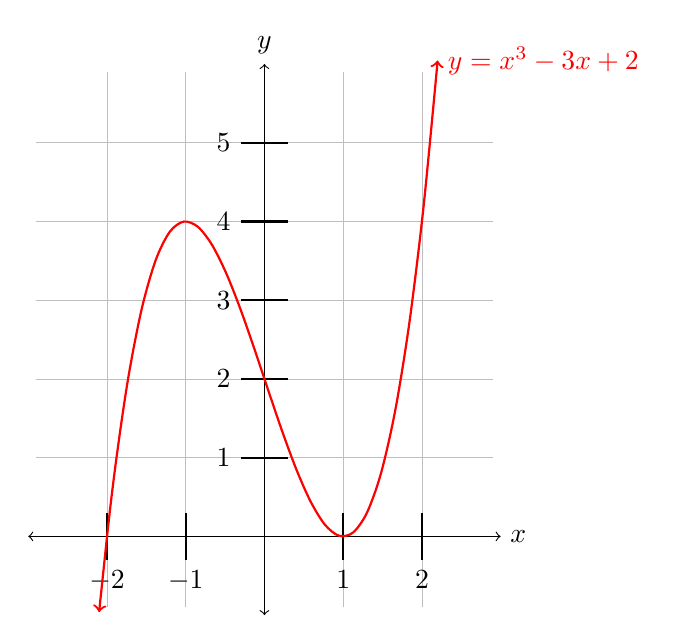
\begin{tikzpicture}[domain=-2.1:2.2,scale=1,smooth]
      \draw[very thin,color=gray!50] (-2.9,-0.9) grid (2.9,5.9);
        
      \draw[<->] (-3,0) -- (3,0) node[right] {$x$};
      \draw[<->] (0,-1) -- (0,6) node[above] {$y$};
      \draw[thick] (1,0.3) -- (1,-0.3) node[below] {1};
      \draw[thick] (2,0.3) -- (2,-0.3) node[below] {2};
      \draw[thick] (-1,0.3) -- (-1,-0.3) node[below] {$-1$};
      \draw[thick] (-2,0.3) -- (-2,-0.3) node[below] {$-2$};
      
      \draw[thick] (0.3,1) -- (-0.3,1) node[left] {1};
      \draw[thick] (0.3,2) -- (-0.3,2) node[left] {2};
      \draw[thick] (0.3,3) -- (-0.3,3) node[left] {3};
      \draw[thick] (0.3,4) -- (-0.3,4) node[left] {4};
      \draw[thick] (0.3,5) -- (-0.3,5) node[left] {5};
        
      \draw[color=red,<->,thick] plot(\x,{(\x)^3-3*(\x)+2}) node[right] {$y=x^3-3x+2$};
    \end{tikzpicture}
  \end{center}
  Which of the following parametric equations yields the same graph?
  \begin{enumerate}[label=\alph*)]
    \item
    $x=\sin t, \ y=\sin^3 t-3\sin t+2$
    \item
    $x=t^3, \ y=t^9-3t^3+2$
    \item
    $x=t^4, \ y=t^{12}-3t^4+2$
    \item
    I don't know
  \end{enumerate}
  \begin{solution}
    b) $x=t^3, \ y=t^9-3t^3+2$
    
    In all three cases, a substitution does yield the equation $y=x^3-3x+2$. But note that with the original function $y=x^3-3x+2$, $x$ can take any real value. So in order to get the entire curve, we must choose parametric equations where $x$ can take any real value. That's not true for $x=\sin t$ (which only yields $-1\le x\le 1$) or $x=t^4$ (which only yields $x\ge 0$). That leaves $x=t^3$ as the correct choice.
  \end{solution}
  \newpage
  \question
  Below is the graph of the left-half of an ellipse. The center of the ellipse is at $(0,0)$; the horizontal radius is 3, and the vertical radius is 2.
  \begin{center}
    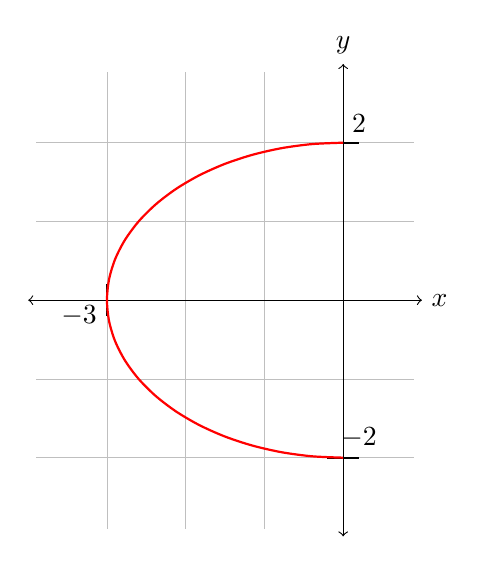
\begin{tikzpicture}[domain=90:270,variable=\t,smooth]
      \draw[very thin,color=gray!50] (-3.9,-2.9) grid (0.9,2.9);
        
      \draw[<->] (-4,0) -- (1,0) node[right] {$x$};
      \draw[<->] (0,-3) -- (0,3) node[above] {$y$};
                
      \draw[thick] (-3,0.2) -- (-3,-0.2) node[below,left] {$-3$};
      \draw[thick] (-0.2,-2) -- (0.2,-2) node[right,above] {$-2$};
      \draw[thick] (-0.2,2) -- (0.2,2) node[right,above] {2};
        
      \draw[color=red,thick] plot({3*cos(\t)},{2*sin(\t)});
        
    \end{tikzpicture}
  \end{center}
  Which of the following parametric equations yields this graph?
  \begin{enumerate}[label=\alph*)]
    \item
    $\displaystyle x=3\cos 2t, \ y=2\sin 2t, \ \frac{\pi}{2}\le t\le\frac{3\pi}{2}$
    \item
    $\displaystyle x=3\cos 3t, \ y=2\sin 3t, \ \frac{5\pi}{6}\le t\le\frac{7\pi}{6}$
    \item
    $\displaystyle x=3\cos 4t, \ y=2\sin 4t, \ 0\le t\le\frac{\pi}{4}$
    \item
    I don't know
  \end{enumerate}
  \begin{solution}
    b) $\displaystyle x=3\cos 3t, \ y=2\sin 3t, \ \frac{5\pi}{6}\le t\le\frac{7\pi}{6}$
    
    All three options do yield the correct overall ellipse. So it comes down to which one yields the correct portion of the ellipse, based on the function being plugged into the sine and cosine (either $2t$, $3t$, or $4t$) and the bounds on the parameter $t$.
    
    For option a), we get:
    $$\pi\le 2t\le 3\pi$$
    That's actually enough for a full loop around the ellipse.
    
    For option c), we get:
    $$0\le 4t\le\pi$$
    That gives us the top-half of the ellipse, instead of the left-half.
    
    For option b), we get:
    $$\frac{5\pi}{2}\le 3t\le\frac{7\pi}{2}$$
    That does give us the left-half of the ellipse, so that is the correct option.
  \end{solution}
  \newpage
  \question
  For which of the following parametric equations is the graph a line segment from $(2,7)$ to $(4,3)$?
  \begin{enumerate}[label=\alph*)]
    \item
    $x=-t+5, \ y=2t+1, \ 3\le t\le 5$
    \item
    $x=t^2-3t+4, \ y=t^2-6t+12, \ 1\le t\le 3$
    \item
    $x=2t+6, \ y=-4t-1, \ -2\le t\le -1$
    \item
    I don't know
  \end{enumerate}
  \begin{solution}
    c) $x=2t+6, \ y=-4t-1, \ -2\le t\le -1$
    
    We know that this choice yields a linear graph because the equations for both $x$ and $y$ are linear. Alternatively, we can rewrite the parametric equations to eliminate the parameter. Solve the first equation for $t$:
    $$t=\frac{1}{2}x-3$$
    Plug that into the second equation, and we end up with a linear function:
    $$y=-4\left(\frac{1}{2}x-3\right)-1$$
    $$y=-2x+12-1$$
    $$y=-2x+11$$
    We can then plug in the least and greatest values for $t$, and make sure we get the endpoints:
    $$t=-2: \ x=2(-2)+6=2, \ y=-4(-2)-1=7$$
    $$t=-1: \ x=2(-1)+6=4, \ y=-4(-1)-1=3$$
    Answer choice a) fails because one of the endpoints is wrong. Answer choice b) fails because the curve isn't even linear. One way to see that: plugging in $t=1$ and $t=3$ does yield the correct endpoints, but plugging in $t=2$ yields the point $(2,4)$, which isn't even on the line segment.
  \end{solution}
  \newpage
  \question
  Given the parametric curve $x=t^2\cos t$, $y=t^3\sin t$, find $\displaystyle\frac{dy}{dx}$.
  \begin{enumerate}[label=\alph*)]
    \item
    $\displaystyle-\frac{3}{2}t\cot t$
    \item
    $\displaystyle\frac{2\cos t-t\sin t}{3t\sin t+t^2\cos t}$
    \item
    $\displaystyle\frac{3t\sin t+t^2\cos t}{2\cos t-t\sin t}$
    \item
    I don't know
  \end{enumerate}
  \begin{solution}
    c) $\displaystyle\frac{3t\sin t+t^2\cos t}{2\cos t-t\sin t}$
    
    $$\frac{dy}{dx}=\frac{dy/dt}{dx/dt}=\frac{3t^2\sin t+t^3\cos t}{2t\cos t+t^2(-\sin t)}=\frac{3t\sin t+t^2\cos t}{2\cos t-t\sin t}$$
  \end{solution}
  \newpage
  \question
  Given the parametric curve $x=t^3+6t$, $y=t^4+4t^2$, find $\displaystyle\frac{d^2 y}{dx^2}$.
  \begin{enumerate}[label=\alph*)]
    \item
    $\displaystyle\frac{6t^2+4}{3t}$
    \item
    $\displaystyle\frac{2}{9t}$
    \item
    $\displaystyle\frac{4}{9t^2+18}$
    \item
    I don't know
  \end{enumerate}
  \begin{solution}
    c) $\displaystyle\frac{4}{9t^2+18}$
    
    $$y'=\frac{dy}{dx}=\frac{dy/dt}{dx/dt}=\frac{4t^3+8t}{3t^2+6}=\frac{4t(t^2+2)}{3(t^2+2)}=\frac{4}{3}t$$
    $$y''=\frac{d^2 y}{dx^2}=\frac{dy'/dt}{dx/dt}=\frac{4/3}{3t^2+6}=\frac{4}{9t^2+18}$$
  \end{solution}
  \newpage
\uplevel{Polar Coordinates}
  \question
  Convert the point $\displaystyle\left(5,\frac{4\pi}{3}\right)$ from polar coordinates to Cartesian coordinates.
  \begin{enumerate}[label=\alph*)]
    \item
    $\displaystyle\left(-\frac{5\sqrt{3}}{2},-\frac{5}{2}\right)$
    \item
    $(-3,-4)$
    \item
    $\displaystyle\left(-\frac{5}{2},-\frac{5\sqrt{3}}{2}\right)$
    \item
    I don't know
  \end{enumerate}
  \begin{solution}
    c) $\displaystyle\left(-\frac{5}{2},-\frac{5\sqrt{3}}{2}\right)$
    
    $$x=r\cos\theta=5\cos\frac{4\pi}{3}=5\cdot\left(-\frac{1}{2}\right)=-\frac{5}{2}$$
    $$y=r\sin\theta=5\sin\frac{4\pi}{3}=5\cdot\left(-\frac{\sqrt{3}}{2}\right)=-\frac{5\sqrt{3}}{2}$$
  \end{solution}
  \newpage
  \question
  Convert the point $(-4,4)$ from Cartesian coordinates to polar coordinates.
  \begin{enumerate}[label=\alph*)]
    \item
    $\displaystyle\left(4\sqrt{2},\frac{3\pi}{4}\right)$
    \item
    $\displaystyle\left(4\sqrt{2},-\frac{\pi}{4}\right)$
    \item
    $\displaystyle\left(8,-\frac{\pi}{4}\right)$
    \item
    I don't know
  \end{enumerate}
  \begin{solution}
    a) $\displaystyle\left(4\sqrt{2},\frac{3\pi}{4}\right)$
    
    $$r=\sqrt{x^2+y^2}=\sqrt{(-4)^2+4^2}=\sqrt{32}=4\sqrt{2}$$
    For the angle, we have $\displaystyle\theta=\tan^{-1}\left(\frac{y}{x}\right)$ for points where $x>0$, but $\displaystyle\theta=\pi+\tan^{-1}\left(\frac{y}{x}\right)$ for points where $x<0$. Thus:
    $$\theta=\pi+\tan^{-1}\left(\frac{4}{-4}\right)=\pi+\tan^{-1}(-1)=\pi+\left(-\frac{\pi}{4}\right)=\frac{3\pi}{4}$$
  \end{solution}
  \newpage
  \question
  Which of the following curves (given in polar form) is a straight line?
  \begin{enumerate}[label=\alph*)]
    \item
    $\displaystyle r=\frac{4}{2\cos\theta+3\sin\theta}$
    \item
    $r=2\theta+3$
    \item
    $r=2\cos\theta+3\sin\theta+4$
    \item
    I don't know
  \end{enumerate}
  \begin{solution}
    a) $\displaystyle r=\frac{4}{2\cos\theta+3\sin\theta}$
    
    Convert this equation from polar coordinates to Cartesian coordinates:
    $$r=\frac{4}{2\cos\theta+3\sin\theta}$$
    $$r(2\cos\theta+3\sin\theta)=4$$
    $$2r\cos\theta+3r\sin\theta=4$$
    $$2x+3y=4$$
    This equation gives us a straight line.    
  \end{solution}
  \newpage
  \question
  Which of the following curves (given in polar form) is a circle?
  \begin{enumerate}[label=\alph*)]
    \item
    $r^2=3\cos\theta+5\sin\theta$
    \item
    $r=3\cos\theta+5\sin\theta$
    \item
    $r=3\cos^2\theta+5\sin^2\theta$
    \item
    I don't know
  \end{enumerate}
  \begin{solution}
    b) $r=3\cos\theta+5\sin\theta$
    
    Convert this equation from polar coordinates to Cartesian coordinates:
    $$r=3\cos\theta+5\sin\theta$$
    $$r^2=3r\cos\theta+5r\sin\theta$$
    $$x^2+y^2=3x+5y$$
    $$x^2+y^2-3x-5y=0$$
    This equation gives us a circle; we could complete the square to find its center and radius.    
  \end{solution}
  \newpage
  \question
  Which of the following curves (given in polar form) does not pass through the origin?
  \begin{enumerate}[label=\alph*)]
    \item
    $r=\sin\theta+2\cos\theta$
    \item
    $r=\sin^2\theta+2\cos^2\theta$
    \item
    $r=\sin^3\theta+2\cos^3\theta$
    \item
    I don't know
  \end{enumerate}
  \begin{solution}
    b) $r=\sin^2\theta+2\cos^2\theta$
    
    The origin is the only point in the plane where $r=0$. So in order for a polar curve to pass through the origin, it must be possible for the value of $r$ to be 0. And that is not possible here:
    $$r=\sin^2\theta+2\cos^2\theta=\sin^2\theta+\cos^2\theta+\cos^2\theta=1+\cos^2\theta\ge 1>0$$
  \end{solution}
  \newpage
  \question
  Which of the following curves (given in polar form) is symmetric about the $x$-axis?
  \begin{enumerate}[label=\alph*)]
    \item
    $r=\cos^2(5\theta)+\sin^3(3\theta)$
    \item
    $r=\cos^3(5\theta)+\sin^2(3\theta)$
    \item
    $r=\cos(1+\theta)+\sin^2\theta$
    \item
    I don't know
  \end{enumerate}
  \begin{solution}
    b) $r=\cos^3(5\theta)+\sin^2(3\theta)$
    
    The two main tests for symmetry about the $x$-axis are replacing $(r,\theta)$ with either $(r,-\theta)$ or $(-r,\pi-\theta)$. In this case, replacing $(r,\theta)$ with $(r,-\theta)$ yields the same equation:
    $$r=\cos^3(-5\theta)+\sin^2(-3\theta)$$
    $$r=\cos^3(5\theta)+(-\sin(3\theta))^2$$
    $$r=\cos^3(5\theta)+\sin^2(3\theta)$$
    Thus, this curve is symmetric about the $x$-axis.
  \end{solution}
  \newpage
  \question
  Which of the following curves (given in polar form) is symmetric about the $y$-axis?
  \begin{enumerate}[label=\alph*)]
    \item
    $r=\theta^5-6\theta^3+4\theta$
    \item
    $r=\theta^7+3\theta^3+1$
    \item
    $r=\theta^4+5\theta^2$
    \item
    I don't know
  \end{enumerate}
  \begin{solution}
    a) $r=\theta^5-6\theta^3+4\theta$
    
    The two main tests for symmetry about the $y$-axis are replacing $(r,\theta)$ with either $(r,\pi-\theta)$ or $(-r,-\theta)$. In this case, replacing $(r,\theta)$ with $(-r,-\theta)$ yields the same equation:
    $$-r=(-\theta)^5-6(-\theta)^3+4(-\theta)$$
    $$-r=-\theta^5+6\theta^3-4\theta$$
    $$-r=-(\theta^5-6\theta^3+4\theta)$$
    $$r=\theta^5-6\theta^3+4\theta$$
    Thus, this curve is symmetric about the $y$-axis.
  \end{solution}
  \newpage
  \question
  Which of the following curves (given in polar form) is symmetric about the origin?
  \begin{enumerate}[label=\alph*)]
    \item
    $r=\cos(3\theta)$
    \item
    $r=\cos(4\theta)$
    \item
    $r=\sin(5\theta)$
    \item
    I don't know
  \end{enumerate}
  \begin{solution}
    b) $r=\cos(4\theta)$
    
    The two main tests for symmetry about the origin are replacing $(r,\theta)$ with either $(r,\pi+\theta)$ or $(-r,\theta)$. In this case, replacing $(r,\theta)$ with $(r,\pi+\theta)$ yields the same equation:
    $$r=\cos(4(\pi+\theta))$$
    $$r=\cos(4\pi+4\theta)$$
    $$r=\cos(4\pi)\cos(4\theta)-\sin(4\pi)\sin(4\theta)$$
    $$r=1\cdot\cos(4\theta)-0\cdot\sin(4\theta)$$
    $$r=\cos(4\theta)$$
    Thus, this curve is symmetric about the origin.
  \end{solution}
  \newpage
\uplevel{Sequences and Series}
  \question
  Which of the following is a formula for the sequence $\{a_n\}=\{4,13,22,31,40,\ldots\}$, where each term is 9 more than the previous term? Assume that the starting value for the index $n$ is 1.
  \begin{enumerate}[label=\alph*)]
    \item
    $\{a_n\}=\{9n-5\}$
    \item
    $\{a_n\}=\{n+9\}$
    \item
    $\{a_n\}=\{9n+4\}$
    \item
    I don't know
  \end{enumerate}
  \begin{solution}
    a) $\{a_n\}=\{9n-5\}$
    
    In general, the sequence $\{rn+s\}$ (starting from $n=1$) gives the sequence whose step size is $r$ and whose first term is $r+s$. The step size here is 9, so $r=9$; then to have the first term be 4, we need $s=-5$.
    
    Note that $9n+4$ would work if the index $n$ started from 0. We could also get something related to $n+9$ if we wrote a recursive formula for the sequence.
  \end{solution}
  \newpage
  \question
  Does the following series converge or diverge? If it converges, find what it converges to.
  $$\sum_{k=2}^\infty 4\cdot\left(-\frac{2}{3}\right)^{k}$$
  \begin{enumerate}[label=\alph*)]
    \item
    Converges to $\displaystyle\frac{16}{15}$
    \item
    Converges to $\displaystyle\frac{12}{5}$
    \item
    Diverges
    \item
    I don't know
  \end{enumerate}
  \begin{solution}
    a) Converges to $\displaystyle\frac{16}{15}$
    
    $$\sum_{k=2}^\infty 4\left(-\frac{2}{3}\right)^{k}=\frac{16}{9}-\frac{32}{27}+\frac{64}{81}-\frac{128}{243}+\cdots$$
    It's a geometric series. The first term is $\displaystyle a=\frac{16}{9}$, and the multiplier is $\displaystyle r=-\frac{2}{3}$. We have $|r|<1$, so the series converges to:
    $$\frac{a}{1-r}=\frac{16/9}{1-(-2/3)}=\frac{16/9}{5/3}=\frac{16}{9}\cdot\frac{3}{5}=\frac{16}{15}$$
  \end{solution}
  \newpage
  \question
  Does the following series converge or diverge? If it converges, find what it converges to.
  $$\sum_{k=1}^\infty 2\cdot\left(-\frac{5}{4}\right)^{k}$$
  \begin{enumerate}[label=\alph*)]
    \item
    Converges to $\displaystyle-\frac{10}{9}$
    \item
    Converges to $\displaystyle\frac{8}{9}$
    \item
    Diverges
    \item
    I don't know
  \end{enumerate}
  \begin{solution}
    c) Diverges
    
    $$\sum_{k=1}^\infty 2\cdot\left(-\frac{5}{4}\right)^{k}=-\frac{5}{2}+\frac{25}{8}-\frac{125}{32}+\cdots$$
    It's a geometric series. The first term is $\displaystyle a=-\frac{5}{2}$, and the multiplier is $\displaystyle r=-\frac{5}{4}$. We have $|r|\ge 1$, so the series diverges.
  \end{solution}
  \newpage
  \question
  Does the following series converge or diverge? If it converges, find what it converges to.
  $$\sum_{k=2}^\infty\left(\frac{1}{\sqrt[3]{k}}-\frac{1}{\sqrt[3]{k+2}}\right)$$
  \begin{enumerate}[label=\alph*)]
    \item
    Converges to $\displaystyle\frac{1}{\sqrt[3]{2}}$
    \item
    Converges to $\displaystyle\frac{1}{\sqrt[3]{2}}+\frac{1}{\sqrt[3]{3}}$
    \item
    Diverges
    \item
    I don't know
  \end{enumerate}
  \begin{solution}
    b) Converges to $\displaystyle\frac{1}{\sqrt[3]{2}}+\frac{1}{\sqrt[3]{3}}$
    
    This is a telescoping series. Let $s_n$ be the partial sum whose final term is $k=n$:
    $$s_n=\left(\frac{1}{\sqrt[3]{2}}-\frac{1}{\sqrt[3]{4}}\right)+\left(\frac{1}{\sqrt[3]{3}}-\frac{1}{\sqrt[3]{5}}\right)+\left(\frac{1}{\sqrt[3]{4}}-\frac{1}{\sqrt[3]{6}}\right)+\cdots+\left(\frac{1}{\sqrt[3]{n}}-\frac{1}{\sqrt[3]{n+2}}\right)$$
    $$=\frac{1}{\sqrt[3]{2}}+\frac{1}{\sqrt[3]{3}}-\frac{1}{\sqrt[3]{n+1}}-\frac{1}{\sqrt[3]{n+2}}$$
    The series converges to $\displaystyle\lim_{n\to\infty}s_n=\frac{1}{\sqrt[3]{2}}+\frac{1}{\sqrt[3]{3}}$.
  \end{solution}
  \newpage
  \question
  Does the following series converge or diverge? If it converges, find what it converges to.
  $$\sum_{k=7}^\infty\left(\frac{6}{k^2-7k+12}\right)$$
  \begin{enumerate}[label=\alph*)]
    \item
    Converges to 2
    \item
    Converges to 6
    \item
    Diverges
    \item
    I don't know
  \end{enumerate}
  \begin{solution}
    a) Converges to 2
    
    First, rewrite this series using partial fractions:
    $$\sum_{k=7}^\infty\left(\frac{6}{k^2-7k+12}\right)=\sum_{k=7}^\infty\left(\frac{6}{(k-4)(k-3)}\right)=\sum_{k=7}^\infty\left(\frac{A}{k-4}+\frac{B}{k-3}\right)$$
    $$6=A(k-3)+B(k-4)$$
    Plug in $k=4$: $6=A$
    
    Plug in $k=3$: $6=B(-1)\rightarrow B=-6$
    
    So the series now looks like this:
    $$\sum_{k=7}^\infty\left(\frac{6}{k-4}-\frac{6}{k-3}\right)$$
    This is a telescoping series. Let $s_n$ be the partial sum whose final term is $k=n$:
    $$s_n=\left(\frac{6}{3}-\frac{6}{4}\right)+\left(\frac{6}{4}-\frac{6}{5}\right)+\left(\frac{6}{5}-\frac{6}{6}\right)+\cdots+\left(\frac{6}{n-4}-\frac{6}{n-3}\right)=\frac{6}{3}-\frac{6}{n-3}$$
    The series converges to $\displaystyle\lim_{n\to\infty}s_n=\frac{6}{3}=2$.
  \end{solution}
  \newpage
  \question
  Does the following series converge or diverge? If it converges, find what it converges to.
  $$\sum_{k=1}^\infty\left(\tan^{-1}k-\tan^{-1}(k+1)\right)$$
  \begin{enumerate}[label=\alph*)]
    \item
    Converges to $\displaystyle-\frac{\pi}{4}$
    \item
    Converges to $\displaystyle\frac{\pi}{4}$
    \item
    Diverges
    \item
    I don't know
  \end{enumerate}
  \begin{solution}
    a) Converges to $\displaystyle-\frac{\pi}{4}$
    
    This is a telescoping series. Let $s_n$ be the partial sum whose final term is $k=n$:
    $$s_n=(\tan^{-1} 1-\tan^{-1} 2)+(\tan^{-1} 2-\tan^{-1} 3)+\cdots+(\tan^{-1} n-\tan^{-1}(n+1))$$
    $$=\tan^{-1} 1-\tan^{-1}(n+1)=\frac{\pi}{4}-\tan^{-1}(n+1)$$
    Now, take the limit:
    $$\lim_{n\to\infty}s_n=\lim_{n\to\infty}\left(\frac{\pi}{4}-\tan^{-1}(n+1)\right)=\frac{\pi}{4}-\frac{\pi}{2}=-\frac{\pi}{4}$$
    This series converges to $\displaystyle-\frac{\pi}{4}$.
  \end{solution}
  \newpage
  \question
  Does the following series converge absolutely, converge conditionally, or diverge?
  $$\sum_{k=2}^\infty\frac{1}{k(\ln k)^{1.5}}$$
  \begin{enumerate}[label=\alph*)]
    \item
    Converges absolutely
    \item
    Converges conditionally
    \item
    Diverges
    \item
    I don't know
  \end{enumerate}
  \begin{solution}
    a) Converges absolutely
    
    With all positive terms, this series either converges absolutely or diverges. Use the Integral Test:
    $$\int_2^\infty\frac{1}{x(\ln x)^{1.5}}\,dx=\lim_{b\to\infty}\int_2^b\frac{1}{x(\ln x)^{1.5}}\,dx$$
    $$u=\ln x; \ du=\frac{1}{x}\,dx$$
    $$x=2\longrightarrow u=\ln 2$$
    $$x=b\longrightarrow u=\ln b$$
    $$\lim_{b\to\infty}\int_{\ln 2}^{\ln b}\frac{1}{u^{1.5}}\,du=\lim_{b\to\infty}\left[\frac{u^{-0.5}}{-0.5}\right]_{\ln 2}^{\ln b}=\lim_{b\to\infty}\left[-\frac{2}{u^{0.5}}\right]_{\ln 2}^{\ln b}$$
    $$=\lim_{b\to\infty}\left[-\frac{2}{(\ln b)^{0.5}}+\frac{2}{(\ln 2)^{0.5}}\right]=\frac{2}{(\ln 2)^{0.5}}$$
      
    The integral $\displaystyle\int_2^\infty\frac{1}{x(\ln x)^{1.5}}\,dx$ converges, so the series $\displaystyle\sum_{k=2}^\infty \frac{1}{k(\ln k)^{1.5}}$ also converges (absolutely).
  \end{solution}
  \newpage
  \question
  Does the following series converge absolutely, converge conditionally, or diverge?
  $$\sum_{k=3}^\infty\frac{1}{k\ln k}$$
  \begin{enumerate}[label=\alph*)]
    \item
    Converges absolutely
    \item
    Converges conditionally
    \item
    Diverges
    \item
    I don't know
  \end{enumerate}
  \begin{solution}
    c) Diverges
        
    With all positive terms, this series either converges absolutely or diverges. Use the Integral Test:
    $$\int_3^\infty\frac{1}{x\ln x}\,dx=\lim_{b\to\infty}\int_3^b\frac{1}{x\ln x}\,dx$$
    $$u=\ln x; \ du=\frac{1}{x}\,dx$$
    $$x=3\longrightarrow u=\ln 3$$
    $$x=b\longrightarrow u=\ln b$$
    $$\lim_{b\to\infty}\int_{\ln 3}^{\ln b}\frac{1}{u}\,du=\lim_{b\to\infty}[\ln|u|]_{\ln 3}^{\ln b}=\lim_{b\to\infty}[\ln(\ln b)-\ln(\ln 3)]=\infty$$
    The integral $\displaystyle\int_3^\infty\frac{1}{x\ln x}\,dx$ diverges, so the series $\displaystyle\sum_{k=3}^\infty\frac{1}{k\ln k}$ also diverges.
  \end{solution}
  \newpage
  \question
  Does the following series converge absolutely, converge conditionally, or diverge?
  $$\sum_{k=1}^\infty\frac{4k^{2.5}}{k^3+17}$$
  \begin{enumerate}[label=\alph*)]
    \item
    Converges absolutely
    \item
    Converges conditionally
    \item
    Diverges
    \item
    I don't know
  \end{enumerate}
  \begin{solution}
    c) Diverges
        
    With all positive terms, this series either converges absolutely or diverges. Use the Limit Comparison Test: compare the given series to $\displaystyle\sum_{k=1}^\infty\frac{4k^{2.5}}{k^3}=\sum_{k=1}^\infty\frac{4}{k^{0.5}}$, which diverges. (It's a $p$-series with exponent at most $1$.)
    $$\lim_{k\to\infty}\frac{\left(\frac{4k^{2.5}}{k^3}\right)}{\left(\frac{4k^{2.5}}{k^3+17}\right)}=\lim_{k\to\infty}\frac{k^3+17}{k^3}=1$$
    We got a positive, finite result, so both series do the same thing. Since $\displaystyle\sum_{k=1}^\infty\frac{4}{k^{0.5}}$ diverges, $\displaystyle\sum_{k=1}^\infty\frac{4k^{2.5}}{k^3+17}$ also diverges.
    
  \end{solution}
  \newpage
  \question
  Does the following series converge absolutely, converge conditionally, or diverge?
  $$\sum_{k=1}^\infty\frac{6k+1}{5k^2+2k^3}$$
  \begin{enumerate}[label=\alph*)]
    \item
    Converges absolutely
    \item
    Converges conditionally
    \item
    Diverges
    \item
    I don't know
  \end{enumerate}
  \begin{solution}
    a) Converges absolutely
        
    With all positive terms, this series either converges absolutely or diverges. Use the Limit Comparison Test: compare the given series to $\displaystyle\sum_{k=1}^\infty\frac{6k}{2k^3}=\sum_{k=1}^\infty\frac{3}{k^2}$, which converges. (It's a $p$-series with exponent greater than $1$.)
    $$\lim_{k\to\infty}\frac{\left(\frac{6k+1}{2k^3+5k^2}\right)}{\left(\frac{3}{k^2}\right)}=\lim_{k\to\infty}\frac{6k^3+k^2}{6k^3+15k^2}=1$$
    We got a positive, finite result, so both series do the same thing. Since $\displaystyle\sum_{k=1}^\infty\frac{3}{k^2}$ converges, $\displaystyle\sum_{k=1}^\infty\frac{6k+1}{5k^2+2k^3}$ also converges (absolutely).    
  \end{solution}
  \newpage
  \question
  Does the following series converge absolutely, converge conditionally, or diverge?
  $$\sum_{k=1}^\infty\frac{\cos^4 k}{k^{1.1}}$$
  \begin{enumerate}[label=\alph*)]
    \item
    Converges absolutely
    \item
    Converges conditionally
    \item
    Diverges
    \item
    I don't know
  \end{enumerate}
  \begin{solution}
    a) Converges absolutely
        
    With all positive terms, this series either converges absolutely or diverges. Use the Direct Comparison Test:
    
    For all $k\ge 1$, we have $0\le\cos^4 k\le 1$. Divide through by $k^{1.1}$, and we get $\displaystyle 0\le\frac{\cos^4 k}{k^{1.1}}\le\frac{1}{k^{1.1}}$. Since $\displaystyle\sum_{k=1}^\infty \frac{1}{k^{1.1}}$ converges (it's a $p$-series with exponent greater than $1$), the lesser series $\displaystyle\sum_{k=1}^\infty\frac{\cos^4 k}{k^{1.1}}$ also converges (absolutely).    
  \end{solution}
  \newpage
  \question
  Does the following series converge absolutely, converge conditionally, or diverge?
  $$\sum_{k=1}^\infty\frac{2+\sin k}{k}$$
  \begin{enumerate}[label=\alph*)]
    \item
    Converges absolutely
    \item
    Converges conditionally
    \item
    Diverges
    \item
    I don't know
  \end{enumerate}
  \begin{solution}
    c) Diverges
        
    With all positive terms, this series either converges absolutely or diverges. Use the Direct Comparison Test:
    
    For all $k\ge 1$, we have $0<1\le 2+\sin k$. Divide through by $k$, and we get $\displaystyle 0<\frac{1}{k}\le\frac{2+\sin k}{k}$. Since $\displaystyle\sum_{k=1}^\infty \frac{1}{k}$ diverges (it's a $p$-series with exponent at most $1$), the greater series $\displaystyle\sum_{k=1}^\infty\frac{2+\sin k}{k}$ also diverges.    
  \end{solution}
  \newpage
  \question
  Does the following series converge absolutely, converge conditionally, or diverge?
  $$\sum_{k=3}^\infty\frac{1}{k^{0.9}(\ln k)^{10}}$$
  \begin{enumerate}[label=\alph*)]
    \item
    Converges absolutely
    \item
    Converges conditionally
    \item
    Diverges
    \item
    I don't know
  \end{enumerate}
  \begin{solution}
    c) Diverges
        
    With all positive terms, this series either converges absolutely or diverges. Use the Direct Comparison Test:
    
    For all sufficiently large $k$, we have $(\ln k)^{10}\le k^{0.01}$. Multiply through by $k^{0.9}$, and we get $k^{0.9}(\ln k)^{10}\le k^{0.91}$. Take reciprocals (which reverses the direction of the inequality when everything is positive), and we get $\displaystyle\frac{1}{k^{0.9}(\ln k)^{10}}\ge\frac{1}{k^{0.91}}\ge 0$. Since $\displaystyle\sum_{k=3}^\infty \frac{1}{k^{0.91}}$ diverges (it's a $p$-series with exponent at most $1$), the series with eventually-greater terms $\displaystyle\sum_{k=3}^\infty\frac{1}{k^{0.9}(\ln k)^{10}}$ also diverges.
  \end{solution}
  \newpage
  \question
  Does the following series converge absolutely, converge conditionally, or diverge?
  $$\sum_{k=2}^\infty\frac{1}{k^{1.2}(\ln k)^3}$$
  \begin{enumerate}[label=\alph*)]
    \item
    Converges absolutely
    \item
    Converges conditionally
    \item
    Diverges
    \item
    I don't know
  \end{enumerate}
  \begin{solution}
    a) Converges absolutely
        
    With all positive terms, this series either converges absolutely or diverges. Use the Direct Comparison Test:
    
    For all sufficiently large $k$, we have $\displaystyle 0\le\frac{1}{k^{1.2}(\ln k)^3}\le\frac{1}{k^{1.2}}$. Since $\displaystyle\sum_{k=2}^\infty \frac{1}{k^{1.2}}$ converges (it's a $p$-series with exponent greater than $1$), the series with eventually-lesser terms $\displaystyle\sum_{k=2}^\infty\frac{1}{k^{1.2}(\ln k)^3}$ also converges (absolutely).
  \end{solution}
  \newpage
  \question
  Does the following series converge absolutely, converge conditionally, or diverge?
  $$\sum_{k=3}^\infty\frac{(-1)^k}{(\ln k)^2}$$
  \begin{enumerate}[label=\alph*)]
    \item
    Converges absolutely
    \item
    Converges conditionally
    \item
    Diverges
    \item
    I don't know
  \end{enumerate}
  \begin{solution}
    b) Converges conditionally
        
    Use the Alternating Series Test to determine convergence:
    
    First, $\displaystyle\frac{1}{(\ln k)^2}>0$ for all $k\ge 3$, so our original series is indeed an alternating series. Second, we have $\displaystyle\frac{1}{(\ln k)^2}>\frac{1}{(\ln(k+1))^2}$ for all $k\ge 3$. And third, we have $\displaystyle\lim_{k\to\infty}\frac{1}{(\ln k)^2}=0$. Because those three things are true, the given series converges.
    
    However, if we take the absolute value of all the terms in the original series, we get $\displaystyle\sum_{k=3}^\infty\frac{1}{(\ln k)^2}$. And that is a divergent series by the Direct Comparison Test; $\displaystyle\frac{1}{(\ln k)^2}>\frac{1}{k}>0$ for all sufficiently large $k$, and $\displaystyle\sum_{k=3}^\infty\frac{1}{k}$ diverges, so $\displaystyle\sum_{k=3}^\infty\frac{1}{(\ln k)^2}$ also diverges.
    
    Thus, $\displaystyle\sum_{k=3}^\infty\frac{(-1)^k}{(\ln k)^2}$ converges conditionally.
  \end{solution}
  \newpage
  \question
  Does the following series converge absolutely, converge conditionally, or diverge?
  $$\sum_{k=0}^\infty(-1)^k\left(\frac{3k^2-8k-14}{20k^2+7k+9}\right)$$
  \begin{enumerate}[label=\alph*)]
    \item
    Converges absolutely
    \item
    Converges conditionally
    \item
    Diverges
    \item
    I don't know
  \end{enumerate}
  \begin{solution}
    c) Diverges
        
    Note that, without the alternating sign, the individual terms of this series do not approach $0$:
    $$\lim_{k\to\infty}\left(\frac{3k^2-8k-14}{20k^2+7k+9}\right)=\frac{3}{20}$$
    Thus, with the alternating sign, the terms do not approach $0$ either (the limit of the individual terms does not exist). So by the Divergence Test, this series diverges.
  \end{solution}  
  \newpage
  \question
  Does the following series converge absolutely, converge conditionally, or diverge?
  $$\sum_{k=2}^\infty\left(\frac{\sin k}{k}+0.5\right)^k$$
  \begin{enumerate}[label=\alph*)]
    \item
    Converges absolutely
    \item
    Converges conditionally
    \item
    Diverges
    \item
    I don't know
  \end{enumerate}
  \begin{solution}
    a) Converges absolutely
    
    Use the Root Test.
    $$\lim_{k\to\infty}\sqrt[k]{|a_k|}=\lim_{k\to\infty}\sqrt[k]{\left|\frac{\sin k}{k}+0.5\right|^k}=\lim_{k\to\infty}\left|\frac{\sin k}{k}+0.5\right|$$
    Note that $\displaystyle\frac{\sin k}{k}$ is approaching 0 here, since the numerator is bounded, and the denominator is approaching infinity. Thus:
    $$\lim_{k\to\infty}\left|\frac{\sin k}{k}+0.5\right|=|0+0.5|=0.5<1$$
    We get something less than 1, so the series converges absolutely.
  \end{solution}
  \newpage
  \question
  Does the following series converge absolutely, converge conditionally, or diverge?
  $$\sum_{k=1}^\infty\left(\frac{8k+5k^2+11}{4k^2+7k+5}\right)^k$$
  \begin{enumerate}[label=\alph*)]
    \item
    Converges absolutely
    \item
    Converges conditionally
    \item
    Diverges
    \item
    I don't know
  \end{enumerate}
  \begin{solution}
    c) Diverges
    
    Use the Root Test.
    $$\lim_{k\to\infty}\sqrt[k]{|a_k|}=\lim_{k\to\infty}\sqrt[k]{\left|\frac{8k+5k^2+11}{4k^2+7k+5}\right|^k}=\lim_{k\to\infty}\left|\frac{8k+5k^2+11}{4k^2+7k+5}\right|$$
    Put the terms in descending order:
    $$\lim_{k\to\infty}\left|\frac{5k^2+8k+11}{4k^2+7k+5}\right|=\frac{5}{4}>1$$
    We get something greater than 1, so the series diverges.
  \end{solution}
  \newpage
  \question
  Does the following series converge absolutely, converge conditionally, or diverge?
  $$\sum_{k=1}^\infty\frac{k^2}{(-1.1)^k}$$
  \begin{enumerate}[label=\alph*)]
    \item
    Converges absolutely
    \item
    Converges conditionally
    \item
    Diverges
    \item
    I don't know
  \end{enumerate}
  \begin{solution}
    a) Converges absolutely
    
    Use the Ratio Test.
    $$\lim_{k\to\infty}\left|\frac{a_{k+1}}{a_k}\right|=\lim_{k\to\infty}\frac{\left|\frac{(k+1)^2}{(-1.1)^{k+1}}\right|}{\left|\frac{k^2}{(-1.1)^k}\right|}=\lim_{k\to\infty}\left(\frac{(k+1)^2}{(1.1)^{k+1}}\right)\left(\frac{(1.1)^k}{k^2}\right)$$
    $$=\lim_{k\to\infty}\frac{(k+1)^2}{1.1k^2}=\lim_{k\to\infty}\frac{k^2+2k+1}{1.1k^2}=\frac{1}{1.1}<1$$
    We get something less than 1, so the series converges absolutely.
  \end{solution}
  \newpage
  \question
  Does the following series converge absolutely, converge conditionally, or diverge?
  $$\sum_{k=1}^\infty\frac{k!}{100^k}$$
  \begin{enumerate}[label=\alph*)]
    \item
    Converges absolutely
    \item
    Converges conditionally
    \item
    Diverges
    \item
    I don't know
  \end{enumerate}
  \begin{solution}
    c) Diverges
    
    Use the Ratio Test.
    $$\lim_{k\to\infty}\left|\frac{a_{k+1}}{a_k}\right|=\lim_{k\to\infty}\frac{\left|\frac{(k+1)!}{100^{k+1}}\right|}{\left|\frac{k!}{100^k}\right|}=\lim_{k\to\infty}\left(\frac{(k+1)!}{100^{k+1}}\right)\left(\frac{100^k}{k!}\right)=\lim_{k\to\infty}\frac{k+1}{100}=\infty>1$$
    We get something greater than 1, so the series diverges.
  \end{solution}
  \newpage
  \question
  Find the interval of convergence of $\displaystyle\sum_{n=1}^\infty\frac{1}{n(-5)^n}(x+3)^n$.
  \begin{enumerate}[label=\alph*)]
    \item
    $\displaystyle\left[-\frac{16}{5},-\frac{14}{5}\right]$
    \item
    $(-8,2]$
    \item
    $[-8,2]$
    \item
    I don't know
  \end{enumerate}
  \begin{solution}
    b) $(-8,2]$
    
    The center of this series is $a=-3$, and the coefficients are $\displaystyle c_n=\frac{1}{n(-5)^n}$ (with $c_0=0$).
    
    Find the radius of convergence:
    $$R=\lim_{n\to\infty}\left|\frac{c_n}{c_{n+1}}\right|=\lim_{n\to\infty}\frac{\left|\frac{1}{n(-5)^n}\right|}{\left|\frac{1}{(n+1)(-5)^{n+1}}\right|}=\lim_{n\to\infty}\frac{(n+1)\cdot 5^{n+1}}{n\cdot 5^n}$$
    $$=\lim_{n\to\infty}\frac{5(n+1)}{n}=\lim_{n\to\infty}\frac{5n+5}{n}=5$$
    The radius of convergence is $5$, so the interval of convergence is $(-8,2)$, possibly including the endpoints.
    
    Check convergence at $x=-8$:
    $$\sum_{n=1}^\infty\frac{1}{n(-5)^n}(-8+3)^n=\sum_{n=1}^\infty\frac{1}{n(-5)^n}(-5)^n=\sum_{n=1}^\infty\frac{1}{n}$$
    This is the harmonic series, which diverges.
    
    Check convergence at $x=2$:
    $$\sum_{n=1}^\infty\frac{1}{n(-5)^n}(2+3)^n=\sum_{n=1}^\infty\frac{1}{n(-5)^n}5^n=\sum_{n=1}^\infty\frac{(-1)^n}{n}$$
    This is the alternating harmonic series, which converges.
    
    This power series converges at the right-endpoint but not at the left-endpoint. So, the interval of convergence is $(-8,2]$.
  \end{solution}
  \newpage
  \question
  Find the interval of convergence of $\displaystyle\sum_{n=1}^\infty\frac{(3x-6)^n}{n^2}$.
  \begin{enumerate}[label=\alph*)]
    \item
    $\displaystyle\left[\frac{5}{3},\frac{7}{3}\right]$
    \item
    $(1,3)$
    \item
    $(5,7)$
    \item
    I don't know
  \end{enumerate}
  \begin{solution}
    a) $\displaystyle\left[\frac{5}{3},\frac{7}{3}\right]$
    
    This series can be rewritten as $\displaystyle\sum_{n=1}^\infty\frac{3^n}{n^2}(x-2)^n$. The center of this series is $a=2$, and the coefficients are $\displaystyle c_n=\frac{3^n}{n^2}$ (with $c_0=0$).
    
    Find the radius of convergence:
    $$R=\lim_{n\to\infty}\left|\frac{c_n}{c_{n+1}}\right|=\lim_{n\to\infty}\frac{\left|\frac{3^n}{n^2}\right|}{\left|\frac{3^{n+1}}{(n+1)^2}\right|}=\lim_{n\to\infty}\left(\frac{3^n}{n^2}\right)\left(\frac{(n+1)^2}{3^{n+1}}\right)$$
    $$=\lim_{n\to\infty}\frac{(n+1)^2}{3n^2}=\lim_{n\to\infty}\frac{n^2+2n+1}{3n^2}=\frac{1}{3}$$
    The radius of convergence is $\displaystyle\frac{1}{3}$, so the interval of convergence is $\displaystyle\left(\frac{5}{3},\frac{7}{3}\right)$, possibly including the endpoints.
    
    Check convergence at $\displaystyle x=\frac{7}{3}$:
    $$\sum_{n=1}^\infty\frac{3^n}{n^2}\left(\frac{7}{3}-2\right)^n=\sum_{n=1}^\infty\frac{3^n}{n^2}\left(\frac{1}{3}\right)^n=\sum_{n=1}^\infty\frac{1}{n^2}$$
    This is a $p$-series with exponent greater than 1; this series converges.
    
    Check convergence at $\displaystyle x=\frac{5}{3}$:
    $$\sum_{n=1}^\infty\frac{3^n}{n^2}\left(\frac{5}{3}-2\right)^n=\sum_{n=1}^\infty\frac{3^n}{n^2}\left(-\frac{1}{3}\right)^n=\sum_{n=1}^\infty\frac{(-1)^n}{n^2}$$
    This series also converges, since if you take the absolute value of all the terms, you get a series that converges (namely, the series for the other endpoint).
    
    Since this power series converges at both endpoints, the interval of convergence is $\displaystyle\left[\frac{5}{3},\frac{7}{3}\right]$.
  \end{solution}
  \newpage
  \question
  Find the interval of convergence of $\displaystyle\sum_{n=0}^\infty\frac{2^n}{n!}(x+5)^n$.
  \begin{enumerate}[label=\alph*)]
    \item
    $\{-5\}$
    \item
    $\displaystyle\left[-\frac{11}{2},-\frac{9}{2}\right]$
    \item
    $(-\infty,\infty)$
    \item
    I don't know
  \end{enumerate}
  \begin{solution}
    c) $(-\infty,\infty)$
    
    The center of this series is $a=-5$, and the coefficients are $\displaystyle c_n=\frac{2^n}{n!}$.
      
    Find the radius of convergence:
    $$R=\lim_{n\to\infty}\left|\frac{c_n}{c_{n+1}}\right|=\lim_{n\to\infty}\frac{\left|\frac{2^n}{n!}\right|}{\left|\frac{2^{n+1}}{(n+1)!}\right|}=\lim_{n\to\infty}\left(\frac{2^n}{n!}\right)\left(\frac{(n+1)!}{2^{n+1}}\right)=\lim_{n\to\infty}\frac{n+1}{2}=\infty$$
    The radius of convergence is $\infty$, so the interval of convergence is the entire real line, $(-\infty,\infty)$.
  \end{solution}
  \newpage
  \question
  Find the interval of convergence of $\displaystyle\sum_{n=0}^\infty\frac{n!}{(-4)^n}(x-7)^n$.
  \begin{enumerate}[label=\alph*)]
    \item
    $\{7\}$
    \item
    $(3,11)$
    \item
    $(-\infty,\infty)$
    \item
    I don't know
  \end{enumerate}
  \begin{solution}
    a) $\{7\}$
    
    The center of this series is $a=7$, and the coefficients are $\displaystyle c_n=\frac{n!}{(-4)^n}$.
      
    Find the radius of convergence:
    $$R=\lim_{n\to\infty}\left|\frac{c_n}{c_{n+1}}\right|=\lim_{n\to\infty}\frac{\left|\frac{n!}{(-4)^n}\right|}{\left|\frac{(n+1)!}{(-4)^{n+1}}\right|}=\lim_{n\to\infty}\left(\frac{n!}{4^n}\right)\left(\frac{4^{n+1}}{(n+1)!}\right)=\lim_{n\to\infty}\frac{4}{n+1}=0$$
    The radius of convergence is 0, so the series only converges at the center point, $a=7$. The interval of convergence is the set containing just that point, $\{7\}$.
  \end{solution}
  \newpage
  \question
  Find the Taylor series (centered at $a=5$) of the function $f(x)=\ln x$.
  \begin{enumerate}[label=\alph*)]
    \item
    $\displaystyle\ln 5+\sum_{n=1}^\infty\frac{(-1)^{n-1}}{n\cdot 5^n}(x-5)^n$
    \item
    $\displaystyle\sum_{n=1}^\infty\frac{(-5)^n}{n}(x-5)^n$
    \item
    $\displaystyle\sum_{n=1}^\infty\frac{(-1)^{n-1}}{n\cdot 5^n}(x-5)^n$
    \item
    I don't know
  \end{enumerate}
  \begin{solution}
    a) $\displaystyle\ln 5+\sum_{n=1}^\infty\frac{(-1)^{n-1}}{n\cdot 5^n}(x-5)^n$
    
    We have $f'(x)=\frac{1}{x}=x^{-1}$, $f''(x)=-x^{-2}$, $f'''(x)=2x^{-3}$,\newline $f^{(4)}(x)=-6x^{-4}$, etc. In general, for $n\ge 1$, we have $$f^{(n)}(x)=(-1)^{n-1}(n-1)!\cdot x^{-n}.$$ So we have $f^{(n)}(5)=(-1)^{n-1}(n-1)!\cdot 5^{-n}$.
      
    Beware: $f^{(0)}(x)=f(x)=\ln x$ does not fit the above pattern. So when we write the Taylor series, we need to write the $n=0$ term separately.
      
    Our Taylor series:
    $$f(x)=\sum_{n=0}^\infty\frac{f^{(n)}(5)}{n!}(x-5)^n=\ln 5+\sum_{n=1}^\infty\frac{(-1)^{n-1}(n-1)!\cdot 5^{-n}}{n!}(x-5)^n$$
    $$=\ln 5+\sum_{n=1}^\infty\frac{(-1)^{n-1}\cdot 5^{-n}}{n}(x-5)^n=\ln 5+\sum_{n=1}^\infty\frac{(-1)^{n-1}}{n\cdot 5^n}(x-5)^n$$
  \end{solution}
  \newpage
  \question
  Find the Maclaurin series of the function $f(x)=4x^7\cos(x^5)$.
  \begin{enumerate}[label=\alph*)]
    \item
    $\displaystyle\sum_{n=0}^\infty\frac{4\cdot(-1)^n}{(2n)!}x^{70n}$
    \item
    $\displaystyle\sum_{n=0}^\infty\frac{4\cdot(-1)^n}{(2n)!}x^{10n+7}$
    \item
    $\displaystyle\sum_{n=0}^\infty\frac{4\cdot(-1)^n}{(2n+1)!}x^{10n+12}$
    \item
    I don't know
  \end{enumerate}
  \begin{solution}
    b) $\displaystyle\sum_{n=0}^\infty\frac{4\cdot(-1)^n}{(2n)!}x^{10n+7}$
    
    Here's the classic Maclaurin series for the function $\cos x$:
    $$\cos x=\sum_{n=0}^\infty\frac{(-1)^n}{(2n)!}x^{2n}$$
    Plug in $x^5$ for $x$:
    $$\cos(x^5)=\sum_{n=0}^\infty\frac{(-1)^n}{(2n)!}(x^5)^{2n}=\sum_{n=0}^\infty\frac{(-1)^n}{(2n)!}x^{10n}$$
    Multiply by $4x^7$:
    $$4x^7\cos(x^5)=\sum_{n=0}^\infty\frac{(-1)^n}{(2n)!}(4x^7)x^{10n}=\sum_{n=0}^\infty\frac{4\cdot(-1)^n}{(2n)!}x^{10n+7}$$
  \end{solution}
  \newpage
  \question
  Find the Maclaurin series of the function $f(x)=7x^2\sin(x^4)$.
  \begin{enumerate}[label=\alph*)]
    \item
    $\displaystyle\sum_{n=0}^\infty\frac{7\cdot(-1)^n}{(2n+1)!}x^{16n+8}$
    \item
    $\displaystyle\sum_{n=0}^\infty\frac{7\cdot(-1)^n}{(2n+1)!}x^{8n+6}$
    \item
    $\displaystyle\sum_{n=0}^\infty\frac{7\cdot(-1)^n}{(2n+1)!}x^{8n+3}$
    \item
    I don't know
  \end{enumerate}
  \begin{solution}
    b) $\displaystyle\sum_{n=0}^\infty\frac{7\cdot(-1)^n}{(2n+1)!}x^{8n+6}$
    
    Here's the classic Maclaurin series for the function $\sin x$:
    $$\sin x=\sum_{n=0}^\infty\frac{(-1)^n}{(2n+1)!}x^{2n+1}$$
    Plug in $x^4$ for $x$:
    $$\sin(x^4)=\sum_{n=0}^\infty\frac{(-1)^n}{(2n+1)!}(x^4)^{2n+1}=\sum_{n=0}^\infty\frac{(-1)^n}{(2n+1)!}x^{8n+4}$$
    Multiply by $7x^2$:
    $$7x^2\sin(x^4)=\sum_{n=0}^\infty\frac{(-1)^n}{(2n+1)!}(7x^2)x^{8n+4}=\sum_{n=0}^\infty\frac{7\cdot(-1)^n}{(2n+1)!}x^{8n+6}$$
  \end{solution}
  \newpage
  \question
  Find the Maclaurin series of the function $\displaystyle f(x)=\int_0^x e^{t^3}\,dt$.
  \begin{enumerate}[label=\alph*)]
    \item
    $\displaystyle\sum_{n=0}^\infty\frac{1}{n!(n+4)}x^{n+4}$
    \item
    $\displaystyle\sum_{n=0}^\infty\frac{1}{n!(3n+1)}x^{3n+1}$
    \item
    $\displaystyle\sum_{n=0}^\infty\frac{1}{n!(3n+3)}x^{3n+3}$
    \item
    I don't know
  \end{enumerate}
  \begin{solution}
    b) $\displaystyle\sum_{n=0}^\infty\frac{1}{n!(3n+1)}x^{3n+1}$
    
    Here's the classic Maclaurin series for the function $e^t$:
    $$e^t=\sum_{n=0}^\infty\frac{1}{n!}t^n$$
    Plug in $t^3$ for $t$:
    $$e^{t^3}=\sum_{n=0}^\infty\frac{1}{n!}(t^3)^n=\sum_{n=0}^\infty\frac{1}{n!}t^{3n}$$
    Integrate:
    $$\int_0^x e^{t^3}\,dt=\sum_{n=0}^\infty\frac{1}{n!}\int_0^x t^{3n}\,dt=\sum_{n=0}^\infty\frac{1}{n!}\left[\frac{t^{3n+1}}{3n+1}\right]_0^x=\sum_{n=0}^\infty\frac{1}{n!(3n+1)}x^{3n+1}$$
  \end{solution}
  \newpage
\end{questions}

\end{document}